\chapter{Metodologia}

Neste capítulo será apresentado a metodologia utilizada para o desenvolvimento
dos objetivos propostos para o projeto. Primeiramente será descrito as etapas
definidas para do desenvolvimento do protocolo, onde cada etapa depende dos
resultados gerados nas etapas anteriores. De modo geral, as etapas podem ser
dividades em 2 fases. A primeira fase de idealização e visão geral, tem o
objetivo de entender e definir o escopo do problema assim como gerar documentações
que vão definir em alto nível o que é, e como funciona o protocolo proposto.
Já na segunda fase, fase de implementação, o objetivo é traduzir toda a
documentação gerada na fase anterior para ser executada e testada num sistema
embarcado. \newline

O processo criativo e de desenvolvimento do sistema proposto seguiu metodologias
inspiradas na literatura de engenharia de software. Para especificar as etapas
segue a Figura \ref{fig:es}.

\begin{figure}[h]
	\begin{center}
	\caption{Etapas do Desenvolvimento do Projeto Proposto}
    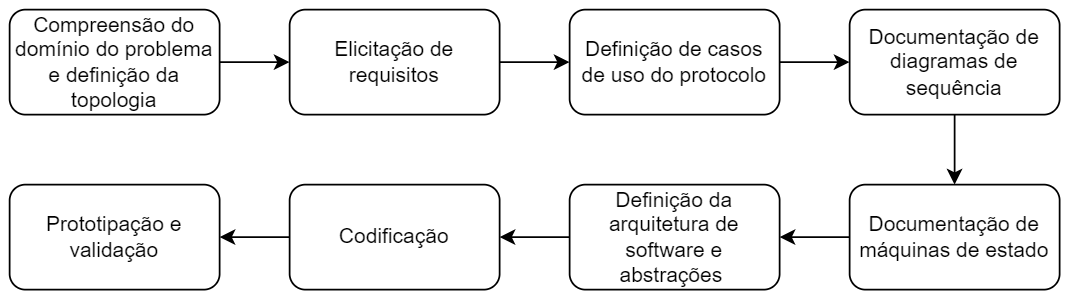
\includegraphics[width=\textwidth]{img/es.drawio.png}
    Fonte: Autor, 2022.
    \label{fig:es}
	\end{center}
\end{figure}

\section{Idealização e Visão Geral}

Vamos supor um cenário onde um desenvolvedor IoT está construindo um sistema
de monitoramento florestal. Ele deseja construir dispositivos embarcados que
monitorem diariamente certo aspecto da floresta e, ao sinal de qualquer mudança,
notifiquem um sistema Web. Porém essa floresta é extremamente remota, longe
de qualquer civilização e, dessa forma, \textbf{longe de fontes de energia e conectividade}.
Assim, ele precisa que seus dispositivos embarcados sejam \textbf{energicamente eficazes},
como também darem suporte para \textbf{enviar e receber mensagens do sistema a longas distâncias}.
O desenvolvedor pesquisa tecnologias no mercado e vê que LoRa pode ser uma solução para
esses problemas. Porém, apenas a adoção de rádios LoRa ao seu projeto não
fornece uma \textbf{infraestrutura de rede preestabelecida} para seus dispositivos, e agora ele se encontra
numa situação onde, além de desenvolver seu projeto principal, ele precisa
implementar alguma arquitetura de rede completa. Tomando esse exemplo como inspiração,
esse trabalho se propõe a
desenvolver um protocolo de rede baseado na tecnologia LoRa que forneça aos
desenvolvedores IoT uma implementação de rede compatível com suas necessidades
genéricas e que seja de fácil integração ao seu projeto atual.

Para definir a topologia da Rede deste projeto é preciso entender que, na maioria das vezes
pela questão remota, poucos dispositivos dessa rede tem a capacidade
de enviar ou receber algum dado pela Internet, logo esses dispositivos precisam
que \textbf{pelo menos 1} dispositivo da rede tenha essa capacidade para que os demais
enviem e recebam suas mensagens do sistema Web por meio deste. Esse dispositivo
recebe um nome especial de \textbf{"Gateway"}, e no geral sua função principal é de ser
essa ponte dos dispositivos locais com a Internet. Já os outros dispositivos recebem o nome de \textbf{"Nó"},
e no geral, é onde se encontra parte das funcionalidades do negócio do
desenvolvedor IoT. Dentre as topologias de Rede existentes, as topologias
\textbf{"Estrela"} e \textbf{"Mesh"} se destacam, cada uma com suas vantagens e desvantagens.
Para esse projeto foi escolhido a topologia Estrela, como pode ser vista
na Figura \ref{fig:topology}, principalmente pela sua simplicidade. Um 
comparativo mais detalhado pode ser visto na Tabela \ref{table:topology}.
\cite{9385408} \cite{9049146} \cite{8115793}

\begin{figure}[h!]
	\begin{center}
	\caption{Topologia de Rede Estrela}
    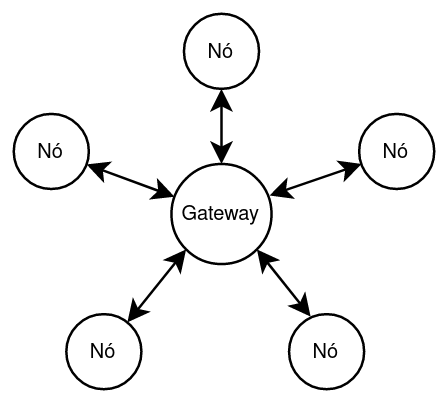
\includegraphics[width=0.31\textwidth]{img/topology.drawio.png}
    
    Fonte: Autor, 2022.
    \label{fig:topology}
	\end{center}
\end{figure}

\begin{table}[h!]
    \begin{center}
    \caption{Comparativo entre Topologia Estrela e Mesh}
    \label{table:topology}
    \begin{tabular}{|l|l|l|}
    \hline
     & Estrela & Mesh \\
    \hline
    Complexidade da Rede & Baixa & Alta \\
    \hline
    Consumo de energia nos Nós & Baixo & Moderado \\
    \hline
    Quantidade máxima de Nós & Máximo suportado pelo Gateway & Soma dos máximos suportados \\
    na Rede                  &                              & pelos dispositivos da Rede \\
    \hline
    Área de cobertura & Distância máxima comum & Soma das distâncias máximas \\
                    &  entre o Gateway e Nós & comuns entre os dispositivos \\
    \hline
    \end{tabular}
    \end{center}
\end{table}

\section{Elicitação de Requisitos}

Pela teoria de engenharia de software, a elicitação de requisitos é uma etapa
em que, ao compreender o escopo do problema, se procura criar uma documento
que descreva certas características que deverá ter na solução, como funcionalidades,
e restrições \cite{324822}. Esse documento contém uma lista de Requisitos
Funcionais e Não-Funcionais e será a primeira documentação formal do
projeto proposto nesse trabalho. Tais requisitos seguiram o padrão que pode
ser visto na Tabela \ref{table:req_model}.

\begin{table}[h]
    \begin{center}
    \caption{Representação de Requisitos Funcionais e Não-Funcionais}
    \label{table:req_model}
    \begin{tabular}{|c|l|}
    \hline
    \textbf{[Identificador Alfanumérico]} & \textbf{Descrição} \\
    \hline
    Nome do Requisito & Texto da Descrição \\
    \hline
    \end{tabular}
    \end{center}
\end{table}

\subsection{Requisitos Funcionais}

Os requisitos funcionais documentados na Tabela \ref{tab:rfs}, descrevem
as funcionalidades que o protocolo proposto nesse trabalho deve possuir. É importante
frisar que esse protocolo tem o objetivo de simplificar o trabalho do desenvolvedor IoT,
como descrito anteriormente, dessa forma o principal usuário do protocolo é a aplicação
do desenvolvedor.


\begin{longtable}{|p{3.5cm}|p{9.0cm}|}
    \caption{Requisitos Funcionais do Protocolo Proposto}\label{tab:rfs} \\
    
    \hline
    \textbf{[RF01]} & \textbf{Descrição} \\
    \hline
    Inicializar em modo de operação de \newline “Nó” & \
    Protocolo dá suporte a uma aplicação para definir seu modo de operação como um Nó na Rede \\
    
    \hline
    \textbf{[RF02]} & \textbf{Descrição} \\
    \hline
    Inicializar em modo de operação de \newline “Gateway” & \
    Protocolo dá suporte a uma aplicação para definir seu modo de operação como um Gateway na Rede \\
    
    \hline
    \textbf{[RF03]} & \textbf{Descrição} \\
    \hline
    Varredura de \newline Gateways ao alcance do Nó & \
    Protocolo dá suporte ao Nó de de fazer uma varredura na sua área de alcance por possíveis Gateways \\
    
    \hline
    \textbf{[RF04]} & \textbf{Descrição} \\
    \hline
    Estabelecer \newline conexão com o \newline Gateway & \
    Protocolo dá suporte ao Nó de estabelecer uma conexão contínua com um Gateway dentro de uma determinada área \\
    \hline
    \newpage
    \hline
    \textbf{[RF05]} & \textbf{Descrição} \\
    \hline
    Suportar \newline múltiplas conexões \newline simultâneas & \
    Protocolo dá suporte a múltiplos Nós conectados ao mesmo tempo num Gateway \\
    
    \hline
    \textbf{[RF06]} & \textbf{Descrição} \\
    \hline
    Suporte ao \newline envio de dados \newline dentro da Rede & \
    Protocolo dá suporte ao envio de dados entre os \newline elementos da rede \\
    
    \hline
    \textbf{[RF07]} & \textbf{Descrição} \\
    \hline
    Suporte ao recebimento de dados \newline dentro da Rede & \
    Protocolo dá suporte ao recebimento de dados entre os elementos da rede \\
    
    \hline
    \textbf{[RF08]} & \textbf{Descrição} \\
    \hline
    Garantia da \newline transmissão \newline dos dados & \
    Protocolo garante que todos os dados enviados irão chegar no destino desde que esteja estabelecida uma conexão durante a transmissão \\
    
    \hline
    \textbf{[RF09]} & \textbf{Descrição} \\
    \hline
    Comunicação entre \newline Nós por meio do \newline Gateway & \
    Protocolo dá suporte aos Nós conectados da Rede de trocarem mensagens entre si por meio do Gateway \\
    
    \hline
    \textbf{[RF10]} & \textbf{Descrição} \\
    \hline
    Verificação de \newline atividade do Nó & \
    Protocolo dá suporte ao Gateway de confirmar o status de “online” do seus clientes \\
    \hline
\end{longtable}

\subsection{Requisitos Não-Funcionais}

Os requisitos não funcionais documentados na Tabela \ref{tab:rnfs}, descrevem
as restrições das funcionalidades do protocolo proposto. Algumas delas impostas
para a simplificação do protocolo, mas uma delas, como a \textbf{[RNF02]}, por
uma limitação física da própria modulação LoRa implementada nos rádios.
\newline
\newline

\begin{longtable}{|p{3.5cm}|p{9.0cm}|}
    \caption{Requisitos Não-Funcionais do Protocolo Proposto}\label{tab:rnfs}\\
    \hline
    \textbf{[RNF01]} & \textbf{Descrição} \\
    \hline
    Dados de \newline tamanho máximo \newline de até 512 bytes & \
    Protocolo exige que o tamanho máximo dos dados trocadas entre elementos da Rede seja de até 512 bytes \\
    \hline
    \textbf{[RNF02]} & \textbf{Descrição} \\
    \hline
    Divisão dos dados em pacotes de até 256 bytes & \
    Protocolo exige que os dados sejam divididos em pacotes de até no máximo de 256 bytes devido a limitação estabelecida pela modulação LoRa \\
    \hline
    \textbf{[RNF03]} & \textbf{Descrição} \\
    \hline
    Máximo de \newline 255 elementos \newline por Rede & \
    Protocolo exige que a quantidade total de elementos numa Rede seja de 255 elementos, onde no máximo 1 Gateway e 254 Nós \\
    \hline
\end{longtable}

\section{Documentação dos Casos de Uso}

Os casos de uso definem as interações, e os objetivos de cada interação, entre atores e sistemas.
Os atores são os principais usuários de um sistema, podem ser desde pessoas até mesmo
programas. De modo geral, um documento de Casos de Uso define quem são os atores do sistema,
de que forma o sistema processa uma interação com os atores, e qual o objetivo das interações
\cite{malan2001functional}. Neste trabalho, o sistema será o protocolo baseado em LoRa,
e o único ator será a aplicação do desenvolvedor IoT, ela que irá usar das funcionalidades
do protocolo para atingir seus objetivos. A figura \ref{fig:use-cases} na página a seguir
apresenta o Diagrama geral de Casos de Uso proposto nesse trabalho. Está seção tem o objetivo
de documentar os Casos de Uso da proposta de acordo com a tabela
\ref{tab:use-cases-def} a seguir.

\begin{longtable}{|p{2.65cm}|l|}
    \caption{Representação dos Casos de Uso}\label{tab:use-cases-def}\\
    \hline
    \textbf{[Identificador]} & Nome do Caso de Uso \\
    \hline
    \textbf{Descrição} & Descrição sobre o caso de uso \\
    \hline
    \textbf{Atores} & Atores envolvidos na interação \\
    \hline
    \textbf{Pré-condições} & Estado do sistema antes da interação \\
    \hline
    \textbf{Pós-condições} & Estado do sistema após a interação \\
    \hline
    \textbf{Fluxo Normal} & Processamento principal da interação \\
    \hline
    \textbf{Fluxos Alt.} & Processamentos alternativos da interação \\
    \hline
    \textbf{RF Rel.} & Requisito implementado pelo caso de uso \\
    \hline
\end{longtable}

\newpage

\begin{figure}[htp]
    \centering
	\caption{Diagrama de Casos de Uso da proposta}
    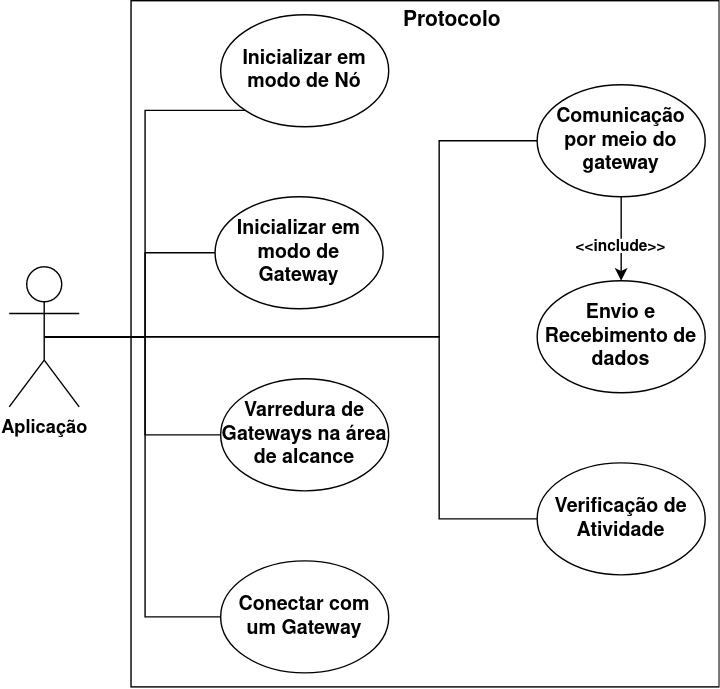
\includegraphics[width=0.6\textwidth,height=0.6\textheight,keepaspectratio]{img/use-cases.drawio.png}
    
    Fonte: Autor, 2022.
    \label{fig:use-cases}
\end{figure}

\begin{longtable}{|p{2.65cm}|p{13cm}|}
    \caption{Caso de Uso UC01}\label{tab:use-cases01} \\
    \hline
    \textbf{[UC01]} & Inicializar em modo de operação de Nó \\
    \hline
    \textbf{Descrição} & Aplicação solicita utilizar as funcionalidades do protocolo em modo de Nó. \\
    \hline
    \textbf{Atores} & Aplicação \\
    \hline
    \textbf{Pré-condições} & Nenhuma. \\
    \hline
    \textbf{Pós-condições} & 1. Protocolo informa que a inicialização foi bem sucedida. \\
    \hline
    \textbf{Fluxo Normal} & 1. Aplicação solicita ao protocolo a inicialização em modo de Nó, fornece seu 
    identificador único (UID) e a interface do rádio LoRa utilizado. \newline
    2. Protocolo informa que a inicialização em modo de Nó foi bem sucedida. \\
    \hline
    \textbf{Fluxos Alt.} & \
    Nenhum. \\
    \hline
    \textbf{RF Rel.} & \
    \textbf{RF01} \\
    \hline
\end{longtable}

\begin{longtable}{|p{2.65cm}|p{13cm}|}
    \caption{Caso de Uso UC02}\label{tab:use-cases02} \\
    \hline
    \textbf{[UC02]} & Inicializar em modo de operação de Gateway \\
    \hline
    \textbf{Descrição} & Aplicação solicita utilizar as funcionalidades do protocolo em modo de Gateway. \\
    \hline
    \textbf{Atores} & Aplicação \\
    \hline
    \textbf{Pré-condições} & Nenhuma. \\
    \hline
    \textbf{Pós-condições} & 1. Protocolo informa que a inicialização foi bem sucedida. \\
    \hline
    \textbf{Fluxo Normal} & 1. Aplicação solicita ao protocolo a inicialização em modo de Gateway, fornece seu identificador único (UID) e a interface do rádio LoRa utilizado. \newline
    2. Protocolo informa que a inicialização em modo de Gateway foi bem sucedida. \\
    \hline
    \textbf{Fluxos Alt.} & Nenhum. \\
    \hline
    \textbf{RF Rel.} & \textbf{RF02} \\
    \hline
\end{longtable}

\begin{longtable}{|p{2.65cm}|p{13cm}|}
    \caption{Caso de Uso UC03}\label{tab:use-cases03} \\
    \hline
    \textbf{[UC03]} & Varredura de Gateways na área de alcance \\
    \hline
    \textbf{Descrição} & Aplicação solicita ao Protocolo para fazer uma varredura de gateways na sua área de alcance. \\
    \hline
    \textbf{Atores} & Aplicação \\
    \hline
    \textbf{Pré-condições} & Protocolo deve ter sido inicializado em modo de Nó. \\
    \hline
    \textbf{Pós-condições} & 1. Protocolo fornece uma lista de Gateway ao seu alcance. \newline
    2. Protocolo informa que não há nenhum Gateway ao seu alcance. \\
    \hline
    \textbf{Fluxo Normal} & 1. Aplicação solicita ao Protocolo para fazer uma varredura por Gateways. \newline
    2. Protocolo no Nó envia um broadcast de um sinal solicitando a identificação dos gateways dentro do seu alcance e aguarda a resposta durante um determinado tempo. \newline
    3. Protocolo no Gateway recebe o broadcast e responde informando sua identificação. \newline
    4. Protocolo no Nó recebe como resposta do seu broadcast a identificação de cada Gateway ao seu alcance. \newline
    5. Protocolo no Nó fornece para a aplicação a lista de identificações dos Gateways ao seu alcance.\\
    \hline
    \textbf{Fluxos Alt.} & 3a. Se o Protocolo no Nó não recebe nenhuma resposta dentro do tempo esperado: \newline
    4a. Nó repete o passo 2 mais uma vez. \newline
    5a. Se novamente não for recebido nenhuma resposta: \newline
    6a. Protocolo no Nó informa que não há nenhum Gateway ao seu alcance. \\
    \hline
    \textbf{RF Rel.} & \textbf{RF03} \\
    \hline
\end{longtable}

\begin{longtable}{|p{2.65cm}|p{13cm}|}
    \caption{Caso de Uso UC04}\label{tab:use-cases04} \\
    \hline
    \textbf{[UC04]} & Conectar com um Gateway \\
    \hline
    \textbf{Descrição} & Aplicação Cliente solicita ao Protocolo para estabelecer conexão com um Gateway, e Aplicação Gateway recebe a nova conexão. \\
    \hline
    \textbf{Atores} & Aplicação Cliente e Aplicação Gateway \\
    \hline
    \textbf{Pré-condições} & Protocolo no Cliente deve ter sido inicializado em modo de Nó. \newline
    Protocolo no Gateway deve ter sido inicializado em modo de Gateway. \\
    \hline
    \textbf{Pós-condições} & 1. Protocolo no Cliente informa que a conexão foi estabelecida, e Protocolo no Gateway informa sobre a nova conexão. \newline
    2. Protocolo no Cliente informa que a conexão não foi estabelecida. \newline
    3. Protocolo no Cliente informa que o Gateway se encontra cheio. \\
    \hline
    \textbf{Fluxo Normal} & 1. Aplicação Cliente solicita ao Protocolo para conectar no Gateway com um identificação determinada. \newline
    2. Protocolo no Cliente envia um sinal de solicitação de conexão para o Gateway e fica no aguardo de uma resposta durante um determinado tempo. \newline
    3. Protocolo no Gateway recebe o sinal e verifica se pode aceitar a conexão. \newline
    4. Protocolo no Gateway responde ao sinal aceitando a conexão, envia o novo identificador de rede do Cliente e fica no aguardo de uma confirmação durante um determinado tempo. \newline
    5. Protocolo no Cliente recebe o sinal, atualiza o seu novo identificador da Rede, e confirma a atualização para o Gateway. \newline
    6. Protocolo no Cliente informa a Aplicação que a conexão foi estabelecida. \newline
    7. Protocolo no Gateway informa ao Gateway sobre a nova conexão. \\
    \hline
    \textbf{Fluxos Alt.} & 2a. Se o Protocolo no Cliente não recebe nenhuma resposta dentro do tempo esperado: \newline
    3a. Nó repete o passo 2 mais uma vez. \newline
    4a. Se novamente não for recebido nenhuma resposta, protocolo no Cliente informa a Aplicação
    que a conexão não foi estabelecida.
    \newline \newline \ 
    4b. Se o Protocolo no Gateway informar ao Cliente que está cheio: \newline
    5b. Protocolo no Cliente informa a Aplicação que o Gateway se encontra cheio no momento. \\
    \hline
    \textbf{RF Rel.} & \textbf{RF04} e \textbf{RF05} \\
    \hline
\end{longtable}

\begin{longtable}{|p{2.65cm}|p{13cm}|}
    \caption{Caso de Uso UC05}\label{tab:use-cases05} \\
    \hline
    \textbf{[UC05]} & Envio e Recebimento de dados \\
    \hline
    \textbf{Descrição} & Aplicação do Remetente solicita ao Protocolo para fazer envio de um dado para um Destinatário na Rede e Aplicação no Destinatário coleta o dado. \\
    \hline
    \textbf{Atores} & Aplicação do Remetente e Aplicação Destinatário \\
    \hline
    \textbf{Pré-condições} & Protocolo deve ter sido inicializado em ambos o Remetente e Destinatário. \newline
    Remetente e Destinatário devem estar conectados ao mesmo Gateway. \\
    \hline
    \textbf{Pós-condições} & 1. Protocolo no Remetente informa para a Aplicação que a transmissão foi bem sucedida e Aplicação Destinatário coleta o novo dado. \newline
    2. Protocolo no Remetente informa que a transmissão não foi bem sucedida. \\
    \hline
    \textbf{Fluxo Normal} & 1. Aplicação Remetente fornece para o Protocolo o dado a ser enviado e o identificador do Destinatário. \newline
    2. Protocolo no Remetente separa o dado em pacotes de tamanho máximo determinado, se necessário. \newline
    3. Protocolo no Remetente envia um pacote para o Protocolo no Destinatário solicitando o envio de dados e informando quantos pacotes serão enviados e aguarda um determinado tempo. \newline
    4. Protocolo no Destinatário recebe a solicitação e verifica se tem recursos sobrando para receber a transmissão. \newline
    5. Protocolo no Destinatário aceita a transmissão e envia um sinal para o Protocolo no Remetente para começar o envio dos pacotes e aguarda um tempo determinado.\newline
    6. Protocolo no Remetente envia pacote e aguarda confirmação de recebimento do Destinatário por um determinado tempo. \newline
    7. Protocolo no Destinatário recebe o pacote e envia confirmação de recebimento ao Remetente e aguarda o próximo pacote por um determinado tempo. \newline
    8. Repete-se o passo 6 ao 7 até que o ultimo pacote seja enviado. \newline
    9. Protocolo no Destinatário, após receber e confirmar o ultimo pacote, reconstrói os dados e informa a Aplicação Destinatário a chegada de novos dados. \newline
    10. Protocolo no Remetente recebe a confirmação do ultimo pacote recebido pelo destinatário e informa a Aplicação Remetente que o envio foi bem sucedido. \\
    \hline
    \textbf{Fluxos Alt.} & 3a. Se o Protocolo no Remetente não recebe uma resposta dentro do tempo determinado: \newline
    4a. Protocolo Remetente repete o passo 3 mais uma vez. \newline
    5a. Se novamente não for recebido nenhuma resposta, Protocolo no Remetente informa a Aplicação Remetente que o envio de dados não foi possível.
    \newline\newline
    4b. Se o Protocolo no Destinatário não tem recursos sobrando para receber a transmissão: \newline
    5b. Protocolo no Destinatário envia um sinal de recursos lotados. \newline
    6b. Protocolo no Remetente recebe a resposta de recursos lotados e informa a Aplicação Remetente que o Destinatário se encontra com recursos ocupados.
    \newline\newline
    6c. Se o Protocolo no Remetente não recebe o sinal de confirmação de recebimento pelo Destinatário: \newline
    7c. Protocolo no Remetente repete o envio do pacote mais uma vez e aguarda um tempo determinado. \newline
    8c. Se novamente não for recebido nenhum resposta, Protocolo no Remetente informa a Aplicação Remetente que o envio de dados não foi possível.
    \newline\newline
    7d. Se o Protocolo no Destinatário não recebe o próximo pacote dentro do tempo esperado: \newline
    8d. Protocolo no Destinatário envia sinal solicitando o reenvio do pacote esperado. \newline
    9d. Se novamente não for recebido nenhum pacote, Protocolo no Destinatário libera recursos alocados para a transmissão. \\
    \hline
    \textbf{RF Rel.} & \textbf{RF06}, \textbf{RF07}, \textbf{RF08} e \textbf{RF09} \\
    \hline
\end{longtable}

\begin{longtable}{|p{2.65cm}|p{13cm}|}
    \caption{Caso de Uso UC06}\label{tab:use-cases06} \\
    \hline
    \textbf{[UC06]} & Verificação de Atividade \\
    \hline
    \textbf{Descrição} & Aplicação Gateway solicita ao protocolo uma verificação de atividade de um determinado Nó. \\
    \hline
    \textbf{Atores} & Aplicação Gateway \\
    \hline
    \textbf{Pré-condições} & Protocolo no Gateway deve ter sido inicializado em modo de Gateway. \newline
    Aplicação Gateway deve ter estabelecido uma conexão com o Nó. \\
    \hline
    \textbf{Pós-condições} & 1. Protocolo no Gateway informa que o Nó está ativo. \newline
    2. Protocolo no Gateway informa que o Nó não está ativo. \\
    \hline
    \textbf{Fluxo Normal} & 1. Aplicação Gateway solicita ao protocolo uma verificação de atividade do Nó com um determinado identificador. \newline
    2. Protocolo no Gateway envia um sinal de verificação para o Nó e fica no aguardo de uma resposta por um determinado tempo. \newline
    3. Protocolo no Nó recebe o sinal e responde confirmando a atividade. \newline
    4. Protocolo no Gateway recebe a confirmação de atividade. \newline
    5. Protocolo no Gateway informa que o Nó está ativo. \\
    \hline
    \textbf{Fluxos Alt.} & 4a. Se o Protocolo no Gateway não recebe a confirmação de atividade: \newline
    5a. Protocolo no Gateway repete o passo 2 mais uma vez \newline
    6a. Se novamente não for recebido nenhuma resposta: \newline
    7a. Protocolo no Gateway informa que o Nó não está ativo. \\
    \hline
    \textbf{RF Rel.} & \textbf{RF10} \\
    \hline
\end{longtable}

\section{Documentação dos Diagramas de Sequência}

O diagrama de sequência é uma ferramenta visual que auxilia o melhor entendimento
das interações definidas na etapa de documentação dos casos de uso. Num diagrama
de sequencia é possível visualizar os fluxos dos casos com mais detalhe numa linha
temporal vertical e os diferentes módulos e atores que estão participando de determinado
fluxo. \newline

Está seção tem objetivo de documentar os diagramas de sequência dos casos de uso estabelecidos
na etapa anterior. A medida em que vamos melhor definindo as interações, mais nos aproximamos
de uma implementação real. Os diagramas a seguir, da Figura \ref{fig:sq-scan} até
\ref{fig:sq-alive-fa}, usam de funções e tipos de mensagens, essas funções e mensagens não
necessariamente representam a sua forma final quando implementada, mas sim tem o intuito
de ajudar o leitor do documento no entendimento do fluxo do diagrama.

\begin{figure}[htp]
    \centering
	\caption{Varredura de Gateways na área de alcance: Fluxo Normal}
    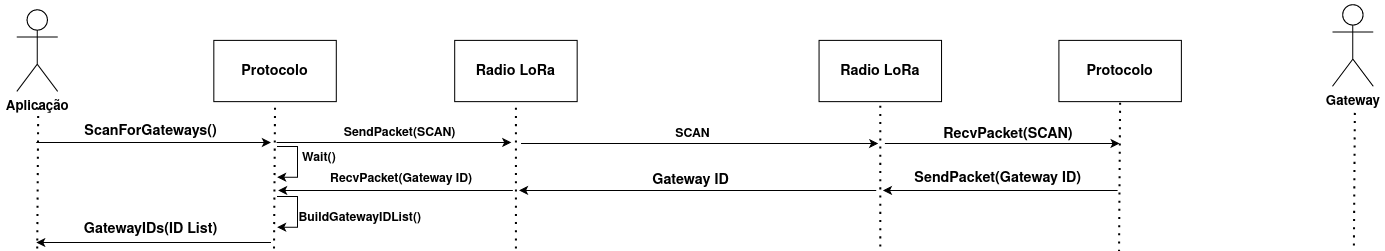
\includegraphics[width=\textwidth,height=0.14\textheight]{img/scan.drawio.png}
    \label{fig:sq-scan}
    Fonte: Autor, 2022.
\end{figure}

Diagrama baseado no caso de uso da tabela \ref{tab:use-cases03}.
\newpage

\begin{figure}[htp]
    \centering
	\caption{Varredura de Gateways na área de alcance: Fluxo Alternativo}
    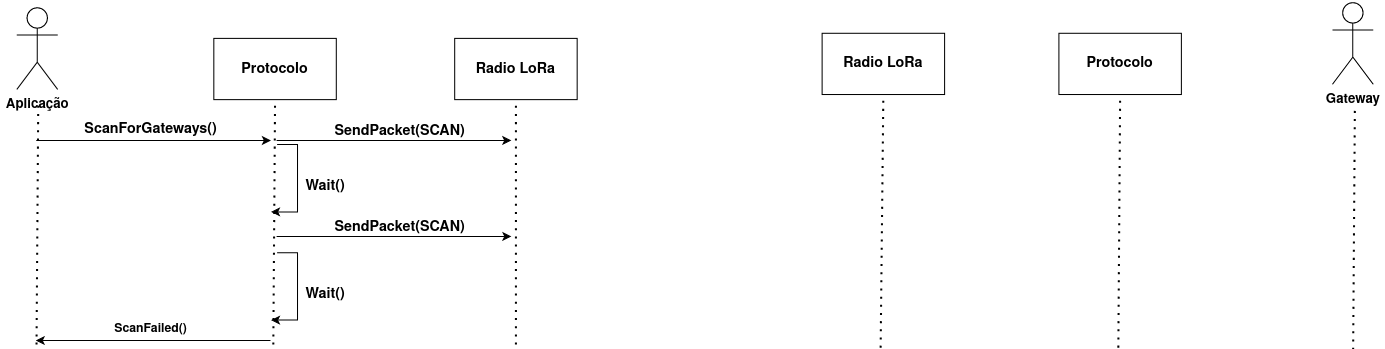
\includegraphics[width=\textwidth,height=0.17\textheight]{img/scan-fa.drawio.png}
    \label{fig:sq-scan-fa}
    Fonte: Autor, 2022.
\end{figure}

Diagrama baseado no caso de uso da tabela \ref{tab:use-cases03}.

\begin{figure}[htp]
    \centering
	\caption{Conectar com um Gateway: Fluxo Normal}
    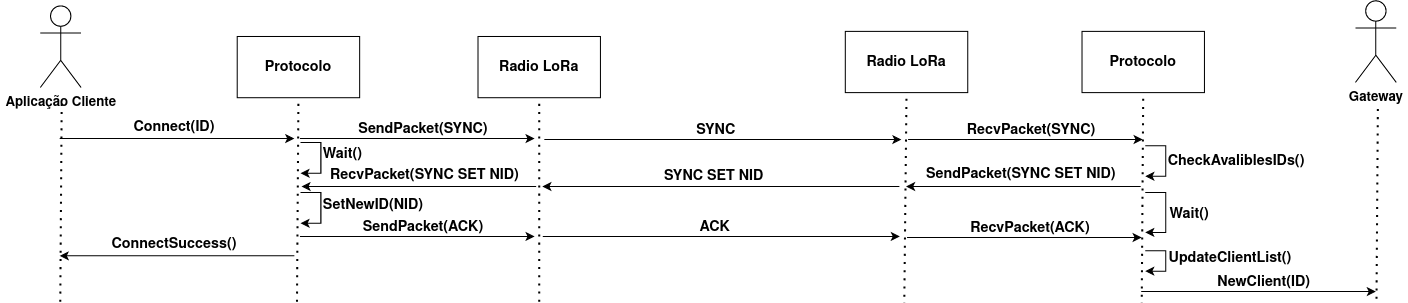
\includegraphics[width=\textwidth,height=0.18\textheight]{img/connect.drawio.png}
    \label{fig:sq-connect}
    Fonte: Autor, 2022.
\end{figure}

Diagrama baseado no caso de uso da tabela \ref{tab:use-cases04}.

\begin{figure}[htp]
    \centering
	\caption{Conectar com um Gateway: Fluxo Alternativo 1}
    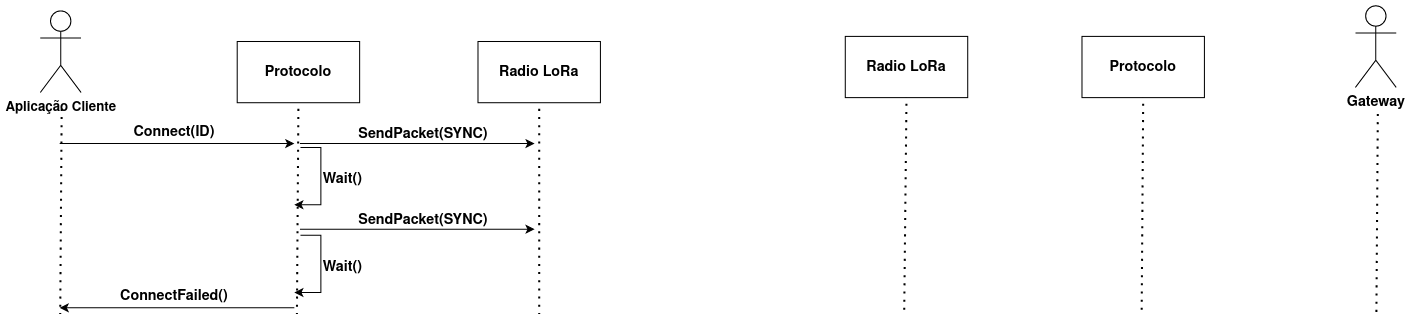
\includegraphics[width=\textwidth,height=0.14\textheight]{img/connect-fa2.drawio.png}
    \label{fig:sq-connect-fa}
    Fonte: Autor, 2022.
\end{figure}

Diagrama baseado no caso de uso da tabela \ref{tab:use-cases04}.
\newpage

\begin{figure}[htp]
    \centering
	\caption{Conectar com um Gateway: Fluxo Alternativo 2}
    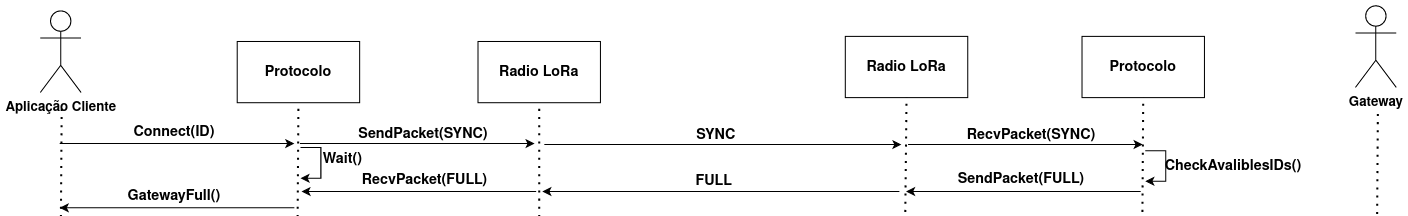
\includegraphics[width=\textwidth,height=0.09\textheight]{img/connect-fa.drawio.png}
    \label{fig:sq-connect-fa2}
    
    Fonte: Autor, 2022.
\end{figure}

Diagrama baseado no caso de uso da tabela \ref{tab:use-cases04}.

\begin{figure}[htp]
    \centering
	\caption{Envio e Recebimento de Dados: Fluxo Normal}
    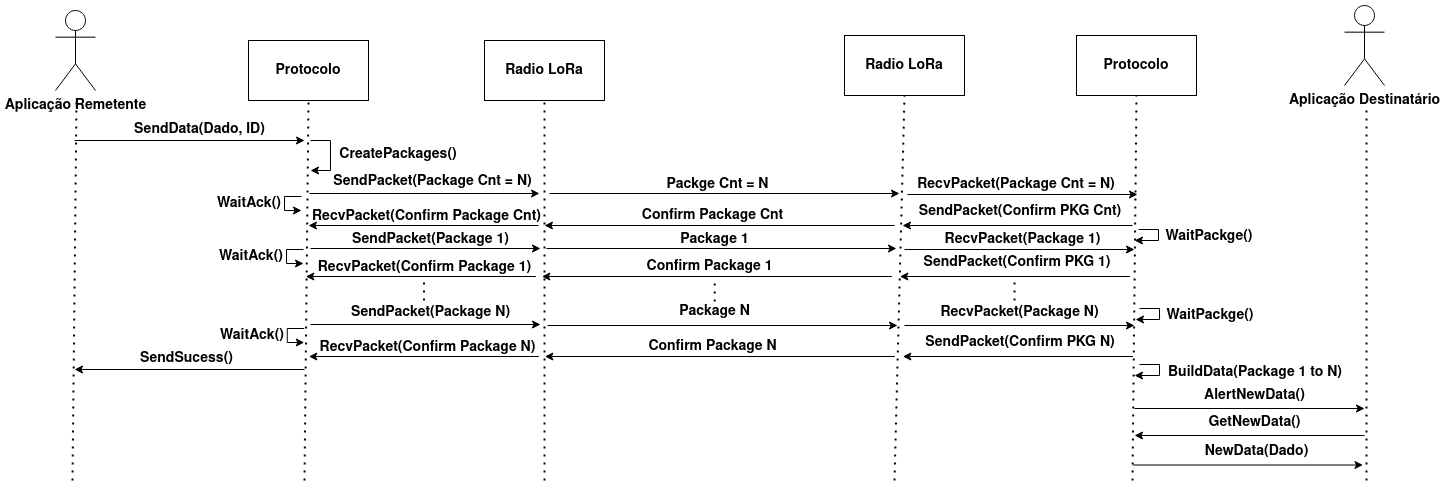
\includegraphics[width=\textwidth,height=0.27\textheight]{img/data.drawio.png}
    \label{fig:sq-data}
    Fonte: Autor, 2022.
\end{figure}

Diagrama baseado no caso de uso da tabela \ref{tab:use-cases05}.

\begin{figure}[htp]
    \centering
	\caption{Envio e Recebimento de Dados: Fluxo Alternativo 1}
    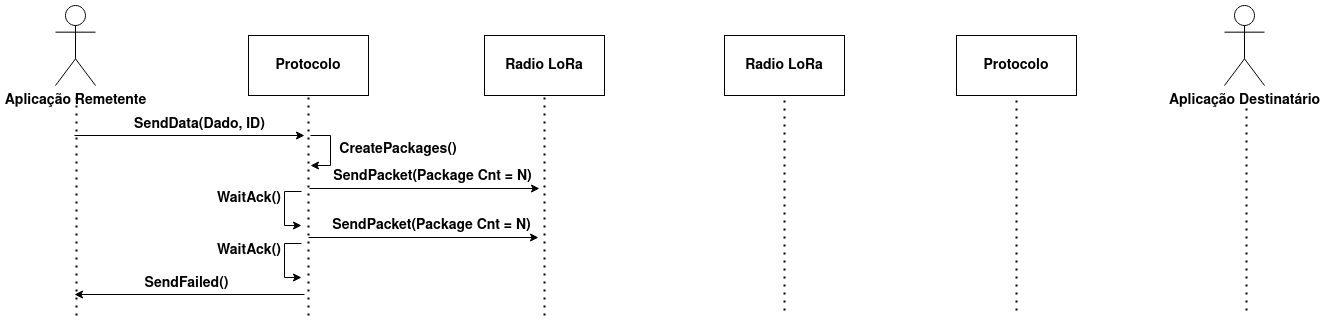
\includegraphics[width=\textwidth,height=0.13\textheight]{img/data-fa.drawio.png}
    \label{fig:sq-data-fa}
    Fonte: Autor, 2022.
\end{figure}

Diagrama baseado no caso de uso da tabela \ref{tab:use-cases05}.
\newpage

\begin{figure}[htp]
    \centering
	\caption{Envio e Recebimento de Dados: Fluxo Alternativo 2}
    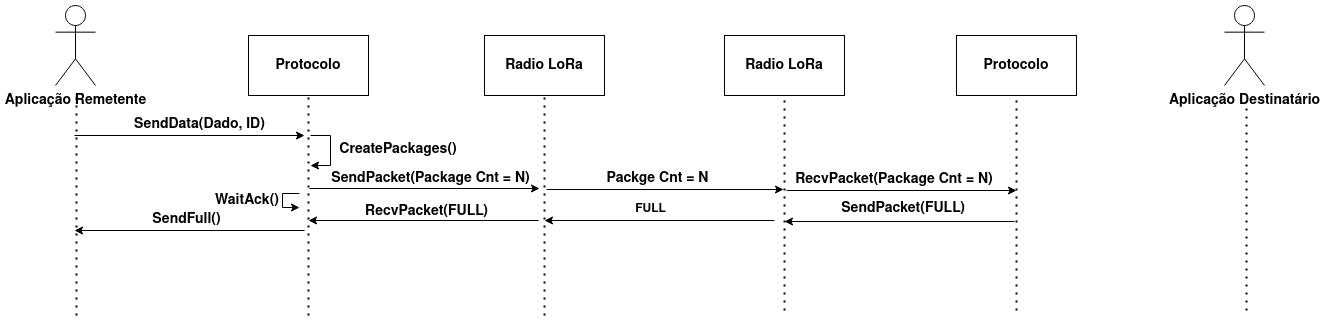
\includegraphics[width=\textwidth]{img/data-fa2.drawio.png}
    \label{fig:sq-data-fa2}
    Fonte: Autor, 2022.
\end{figure}

Diagrama baseado no caso de uso da tabela \ref{tab:use-cases05}.

\begin{figure}[htp]
    \centering
	\caption{Envio e Recebimento de Dados: Fluxo Alternativo 3}
    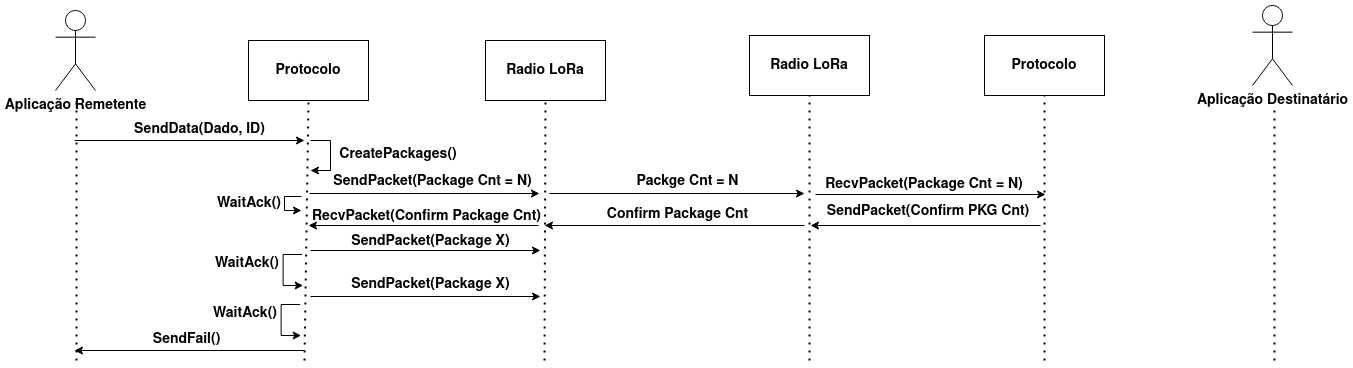
\includegraphics[width=\textwidth]{img/data-fa3.drawio.png}
    \label{fig:sq-data-fa3}
    Fonte: Autor, 2022.
\end{figure}

Diagrama baseado no caso de uso da tabela \ref{tab:use-cases05}.
\newpage

\begin{figure}[htp]
    \centering
	\caption{Envio e Recebimento de Dados: Fluxo Alternativo 4}
    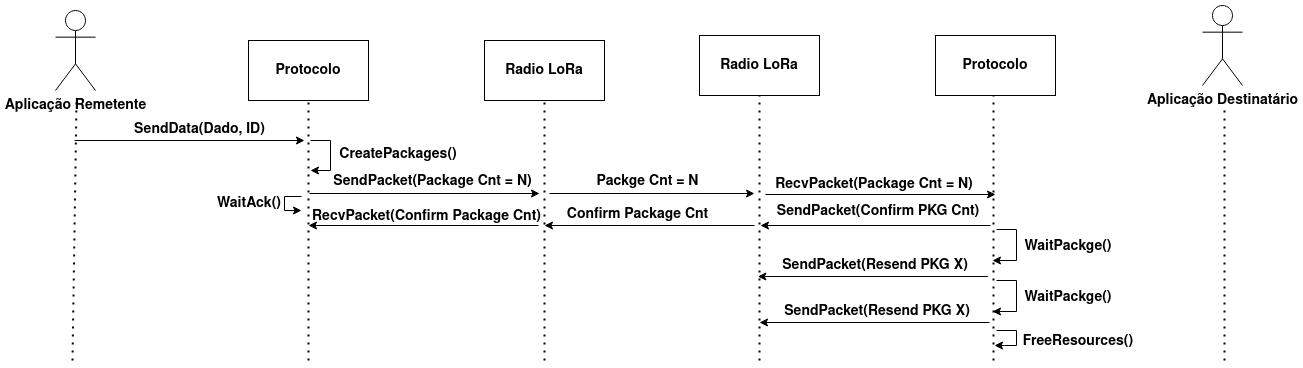
\includegraphics[width=\textwidth]{img/data-fa4.drawio.png}
    \label{fig:sq-data-fa4}
    Fonte: Autor, 2022.
\end{figure}

Diagrama baseado no caso de uso da tabela \ref{tab:use-cases05}.

\begin{figure}[htp]
    \centering
	\caption{Verificação de Atividade: Fluxo Normal}
    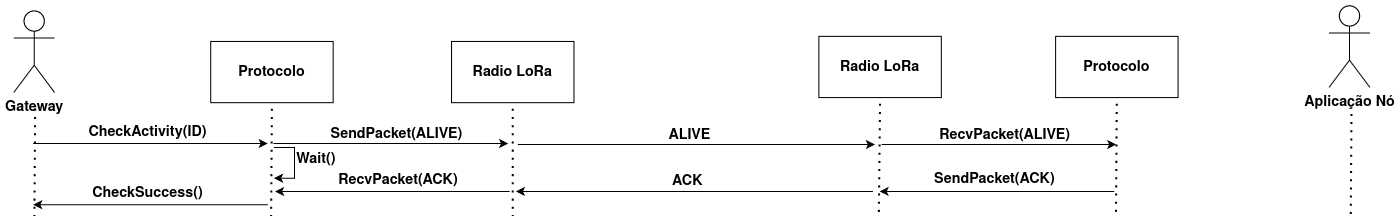
\includegraphics[width=\textwidth]{img/alive.drawio.png}
    \label{fig:sq-alive}
    Fonte: Autor, 2022.
\end{figure}

Diagrama baseado no caso de uso da tabela \ref{tab:use-cases06}.

\begin{figure}[htp]
    \centering
	\caption{Verificação de Atividade: Fluxo Alternativo}
    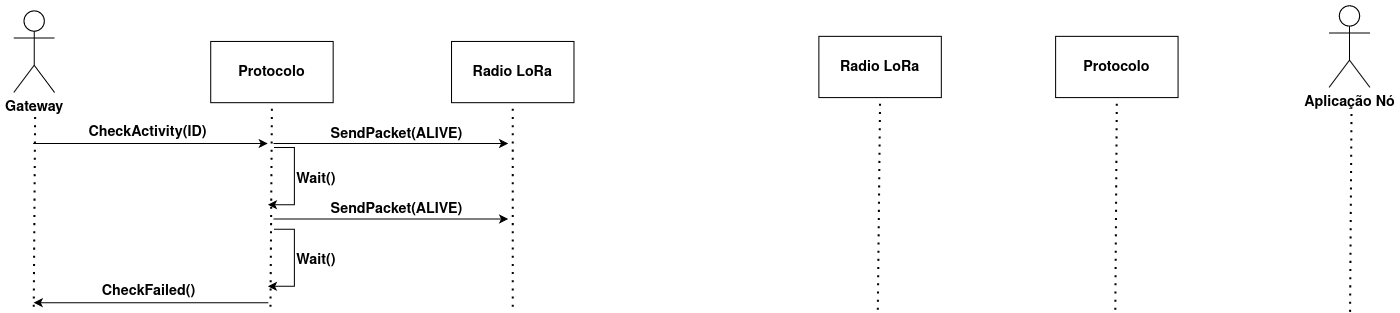
\includegraphics[width=\textwidth]{img/alive-fa.drawio.png}
    \label{fig:sq-alive-fa}
    Fonte: Autor, 2022.
\end{figure}

Diagrama baseado no caso de uso da tabela \ref{tab:use-cases06}.
\newpage

\subsection{Definição do Frame dos Pacotes}

Os diagramas de sequência ajudam a produzir uma etapa muito
importante do projeto que é importante a definição da
estrutura dos pacotes que vão estar trafegando pelos dispositivos da rede.
Dentro pacote é necessário o que chamamos de "metadados", que são
nada mais do que dados que contém informações sobre o pacote.
É graças aos metadados que as máquinas de estado, que serão criadas na próxima etapa,
podem entender que tipo de interação está acontecendo entre os módulos
naquele determinado estado, e dessa maneira, tomar ações. Pelo requisito
não-funcional \textbf{RNF02} os pacotes devem ter tamanho
máximo de até 256 bytes, o que nós da a quantidade de bytes que é preciso dividir
entre os metadados e os dados. Ainda pelos requisitos não-funcionais, o
requisito \textbf{RNF03} define que a Rede pode ter no máximo 255 dispositivos,
dessa forma é precisa no mínimo de 8 bits (1 byte) para identificar unicamente
todos os dispositivos da Rede. Levando essas informações em consideração, e
tomando como inspiração metadados de protocolos já existentes como o IP e MAC,
na figura \ref{fig:frame} e Tabela \ref{tab:metadata}, é apresentado a estrutura
do pacote definida para essa proposta.

\begin{figure}[htp]
    \centering
	\caption{Frame de um Pacote do Protocolo}
    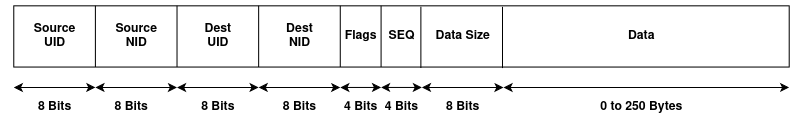
\includegraphics[width=\textwidth]{img/frame.drawio.png}
    \label{fig:frame}
    Fonte: Autor, 2022.
\end{figure}

\begin{longtable}{|l|l|}
    \caption{Detalhamento dos Metadados do Pacote}\label{tab:metadata}\\
    \hline
    Parâmetro & Descrição \\
    \hline
    Source UID & Identificador Único do Remetente \\
    \hline
    Source NID & Identificador de Rede do Remetente \\
    \hline
    Dest UID & Identificador Único do Destinatário \\
    \hline
    Dest NID & Identificador Rede do Destinatário \\
    \hline
    Flags & Tipo do Pacote \\
    \hline
    SEQ & Numero de sequência do Pacote \\
    \hline
    Data Size & Tamanho dos Dados \\
    \hline
\end{longtable}

Os conceitos de UID e NID são importantes pois, da mesma forma em que
um computador ao se conectar numa rede recebe um IP dinâmico do seu Modem, 
no protocolo proposto aqui, o Nó ao se conectar num Gateway receberá um
NID. Dessa forma o protocolo no Gateway pode gerenciar dinamicamente os
clientes da sua rede. Além de que, para o desenvolvedor da aplicação IoT,
o NID do seu dispositivo não importa, mas sim uma forma de poder identificar
um dispositivo especifico dentro da rede, para isso é usado o UID. O UID
é um identificador único restrito ao desenvolvedor, e através dele o desenvolvedor
pode solicitar ao protocolo para enviar dados para um UID especifico. Dessa
forma, os Rádios LoRa se comunicam por meio do NID, e as Aplicações por meio
do UID, um detalhe sútil mas que abre muitas possibilidades e flexibilidades.

\section{Documentação das Máquinas de Estado}

%Esta seção marca a última etapa da primeira fase, descrita anteriormente, de
%idealização e documentação. Ao final, teremos compreendido a problemática e
%produzido documentações baseadas na literatura que definem em alto nível o
%sistema proposto. \newline

A máquina de estado é uma das documentações que mais se aproxima de uma implementação
final. Numa máquina de estado definimos em que ponto se encontra o sistema (Estado
Atual), quais são as ações desse estado, e de que forma é possível de sair
de um estado para outros, além das ações que podem acontecer nas transições entre
estados. De certa formal, é possível visualizar máquinas de estado como
a tradução dos diagramas de sequência para uma lógica programável.

\subsection{Visão Geral}

Foram documentadas nessa proposta duas máquinas de estado, uma para o Gateway
e uma para o Nó. Apesar de distintas, as duas máquinas compartilham fluxos
comuns como o de envio e recebimento de dados, tornando possível construir
uma grande máquina única para os dois modos de operação. Porém, é importante
entender que, ao implementar em hardware, o protocolo em modo Gateway irá
requerer muito mais memória do que o protocolo em modo Cliente, isso se dá
pois o Gateway precisa gerenciar simultaneamente diferentes conexões com diferentes
clientes onde cada uma pode estar em estados distintos da máquina de estado.
Logo trará benefícios mais a frente no desenvolvimento a construção independente 
das máquinas de cada um.
Na Figura \ref{fig:node-fsm} e \ref{fig:gateway-fsm} podemos ter uma visão geral
das máquinas para o Nó e Gateway respectivamente. Nas sub-seções a frente
esse trabalho entrará em melhor detalhes de como os fluxos estão
implementados em cada uma. É importante ressaltar que cada fluxo detalhado foi
baseado nos diagramas de sequência produzidos na etapa anterior.

\clearpage

\begin{figure}[htp]
    \centering
	\caption{Visão Geral da Máquina de Estado do Nó}
    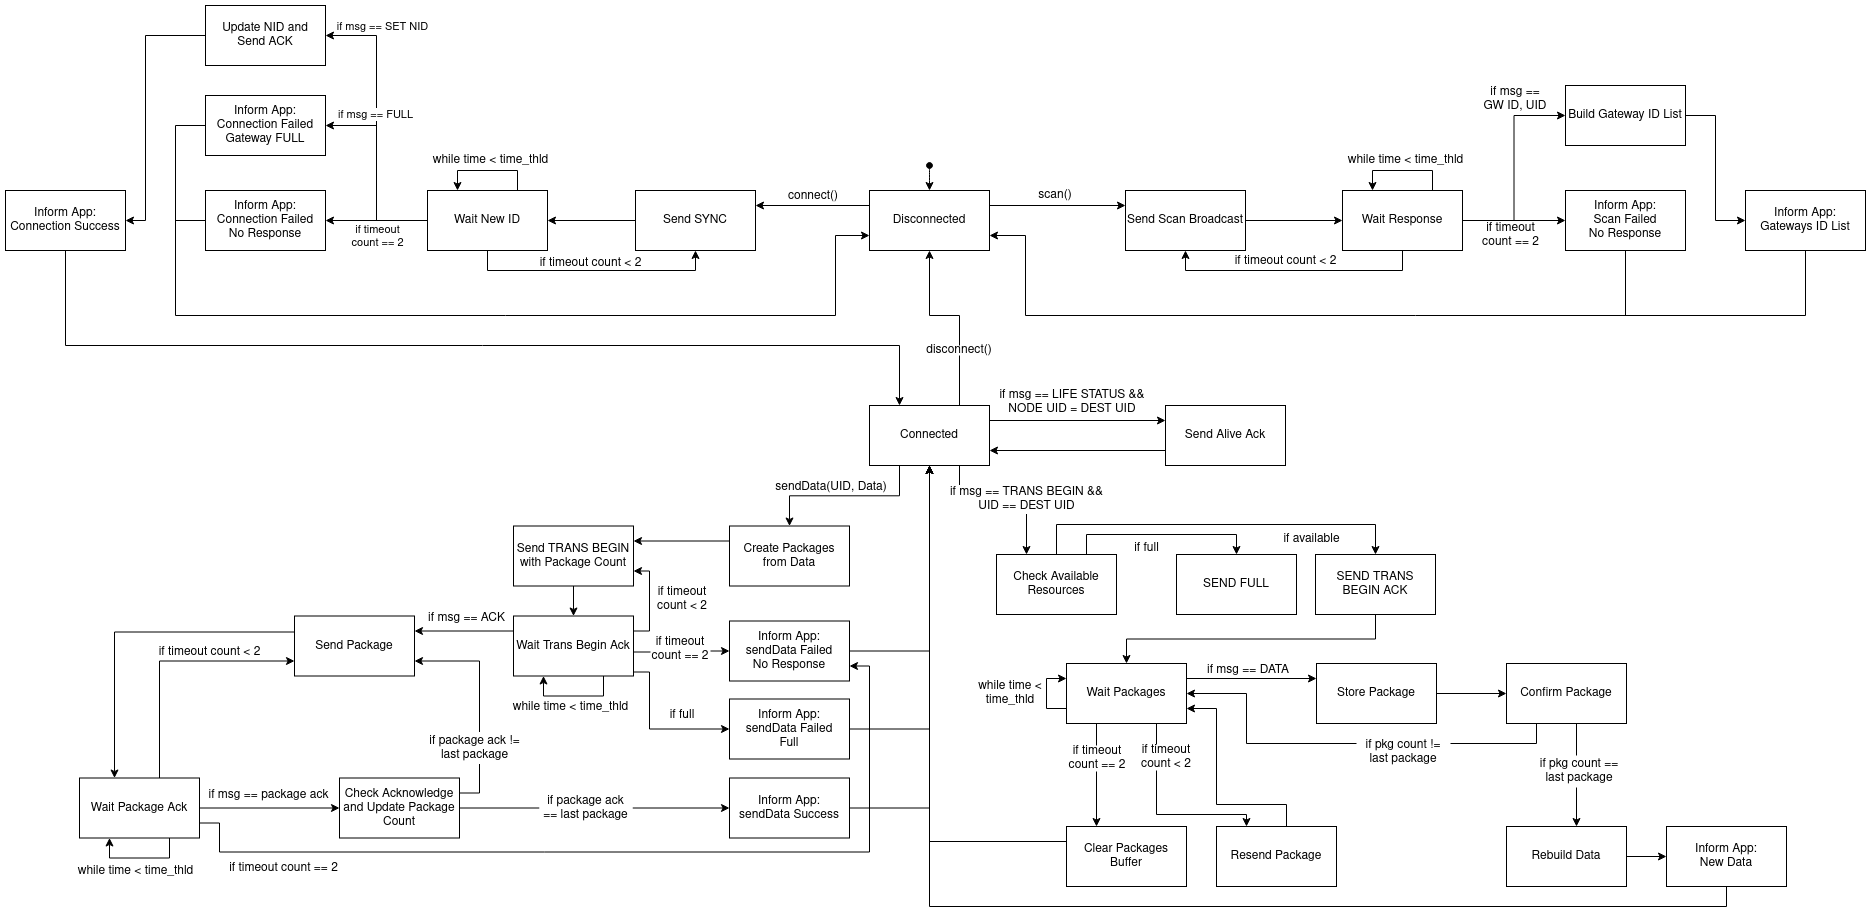
\includegraphics[width=\textwidth,height=0.3\textheight]{img/node_fsm.drawio.png}
    Fonte: Autor, 2022.
    \label{fig:node-fsm}
\end{figure}

\begin{figure}[htp]
    \centering
	\caption{Visão Geral da Máquina de Estado do Gateway}
    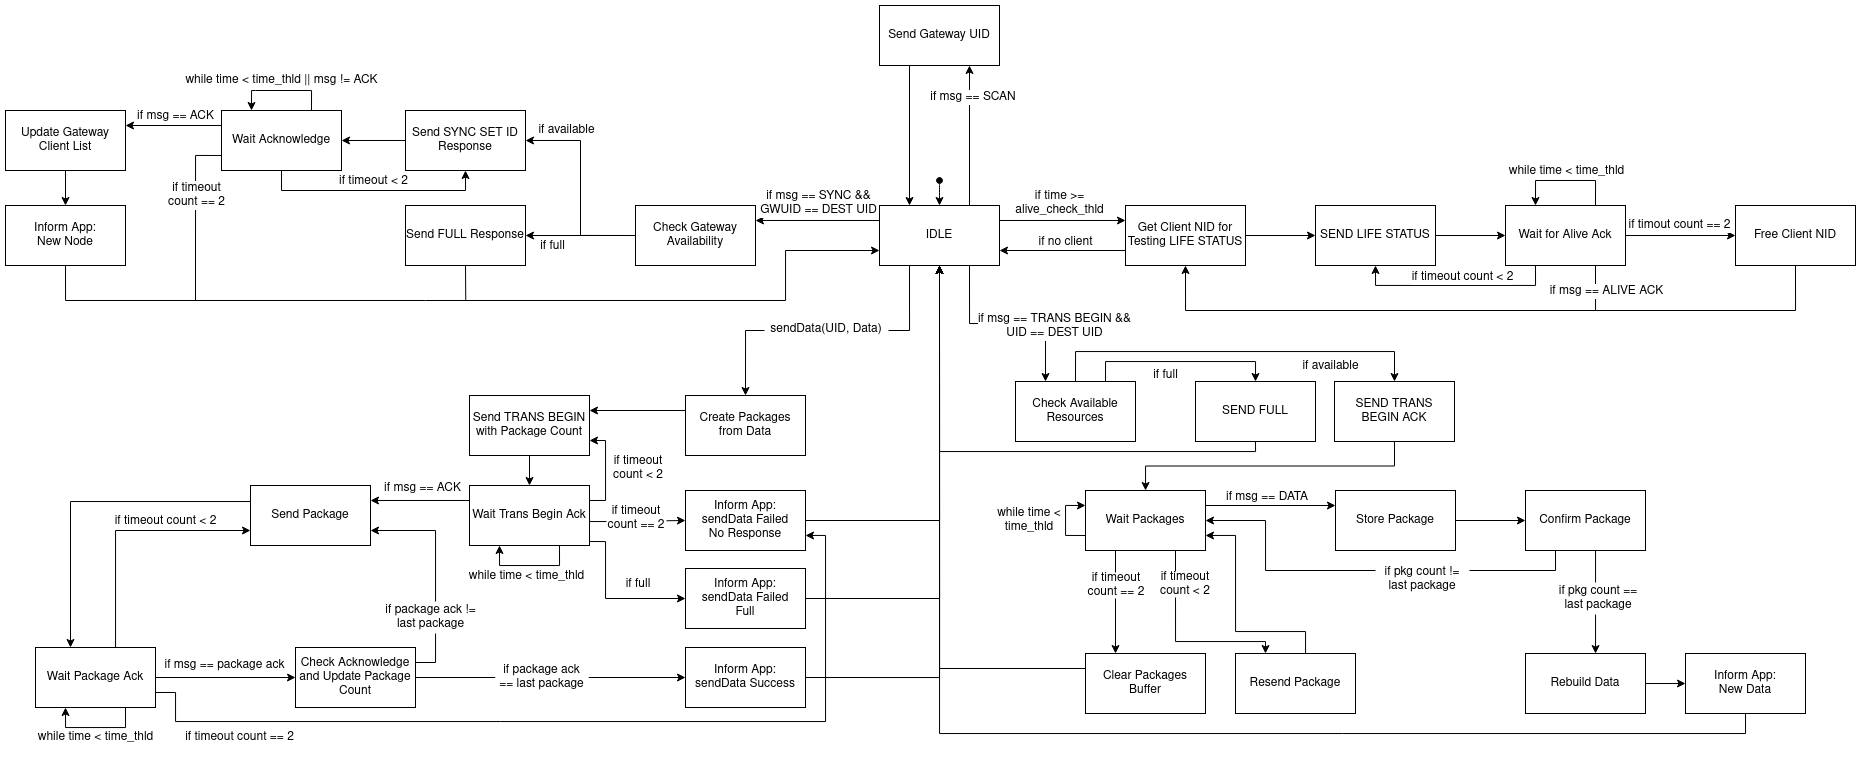
\includegraphics[width=\textwidth,height=0.315\textheight]{img/gateway_fsm.drawio.png}
    Fonte: Autor, 2022.
    \label{fig:gateway-fsm}
\end{figure}

\subsection{Estados de inicialização em Modo de Gateway ou Nó}

Esse fluxo é o mais simples de todos pois ele apenas configurará o
protocolo com o modo de operação devido e inicializará a maquina de estado
adequada. Logo ele não tem uma representação visual
nas máquinas de estado, mas, de certa forma, podem ser considerados
como o estado inicial delas.

\subsection{Estados de Varredura pelo Gateway}

Nesse fluxo, como pode ser visto nas figuras \ref{fig:fsm-node-scan} e \ref{fig:fsm-gw-scan},
o Nó se encontra em seu estado inicial de desconectado.
O objetivo é descobrir se existe algum Gateway na sua área de alcance,
então o Nó vai para o estado de enviar um sinal de varredura, e depois
para o estado de espera de uma resposta. Enquanto isso, um Gateway na
área de alcance e em seu estado inicial de espera recebe o sinal enviado
pelo Nó, logo esse passa para o estado de enviar uma resposta informando
o UID do Gateway presente na área, e depois volta para seu estado de espera
inicial. Ao Nó receber a resposta do Gateway, ele constrói uma lista
dcom o UID do Gateway e vai para o estado de informar a aplicação sobre
a varredura. Caso o Nó não receba nenhuma resposta dentro de um determinado
tempo após o envio do sinal de varredura, ele volta para o estado de envio
e tenta mais uma vez. Caso ainda sim não tenha uma resposta, ele vai para
o estado de informar a aplicação que a varredura não teve respostas.

\begin{figure}[htp]
    \centering
	\caption{Máquina De Estado do Nó: Varredura por Gateways}
    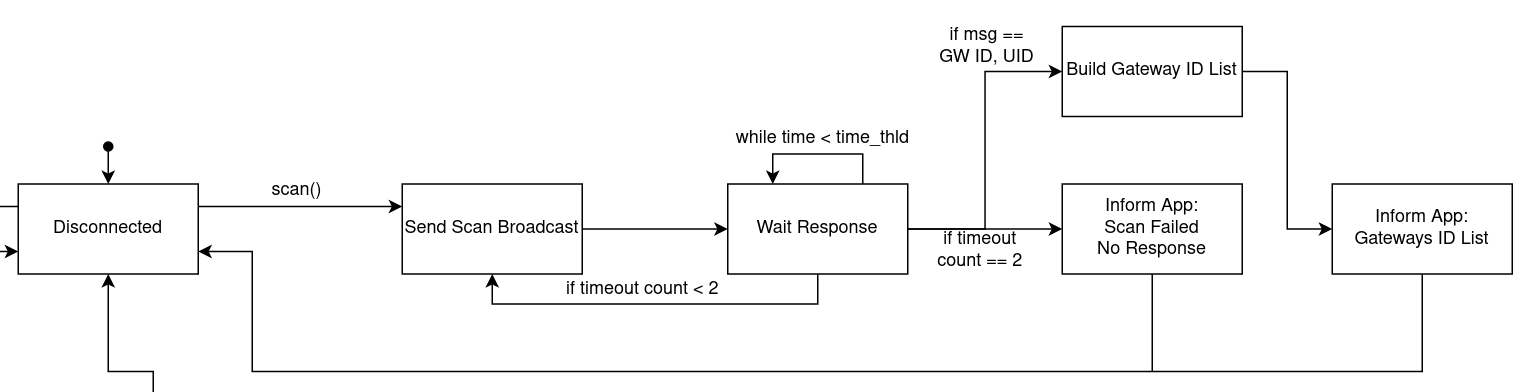
\includegraphics[width=\textwidth]{img/node-scan.drawio.png}
    Fonte: Autor, 2022.
    \label{fig:fsm-node-scan}
\end{figure}

\begin{figure}[htp]
    \centering
	\caption{Máquina De Estado do Gateway: Varredura por Gateways}
    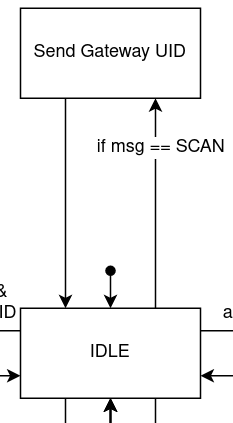
\includegraphics[width=0.15\textwidth]{img/gw-scan.drawio.png}
    
    Fonte: Autor, 2022.
    \label{fig:fsm-gw-scan}
\end{figure}

\subsection{Estados de Conexão com um Gateway}

Feita uma varredura para descobrir os UIDs de Gateways na área de alcance,
o Nó para se conectar vai para o estado de enviar uma sinal de sincronização
junto com o UID do Gateway que deseja conectar. Após o envio, o Nó vai para um
estado de espera por um determinado tempo. No Gateway, ao receber o sinal de sincronização,
é feito a troca de estado para verificar
se existe algum NID livre na Rede para reserva-lo ao Nó que solicitou a conexão.
Caso exista, o Gateway vai para o estado de responder ao Nó com um sinal de atualização para o novo NID
e logo em seguida fica no estado de aguardo da confirmação do Nó.
Caso não exista, ela vai para o estado de responder ao Nó que está com a
quantidade máxima de clientes e volta para o estado de espera. No Nó,
ao receber o sinal de atualização do novo NID, é feito a troca de estado para responder ao Gateway
com uma confirmação de que atualizou seu NID, depois para um estado
de informar a aplicação que a conexão foi bem sucedida e, por fim, o estado
de conectado. Caso o Nó receba o sinal de Gateway cheio, ele vai para
o estado que informa a aplicação que a conexão falhou pois o Gateway está
no limite máximo de clientes. Caso o Nó não receba nenhuma resposta do seu
pedido de sincronização dentro de um determinado tempo, ele volta para
o estado de conexão para tentar mais uma vez. Caso ainda sim, não tenha
resposta, o Nó vai para um estado de informar que a conexão falhou por
falta de resposta e volta para o seu estado de desconectado. Essa descrição pode ser vista nas
figuras \ref{fig:fsm-node-connect} e \ref{fig:fsm-gw-connect}.

\begin{figure}[htp]
    \centering
	\caption{Máquina De Estado do Nó: Conexão com um Gateway}
    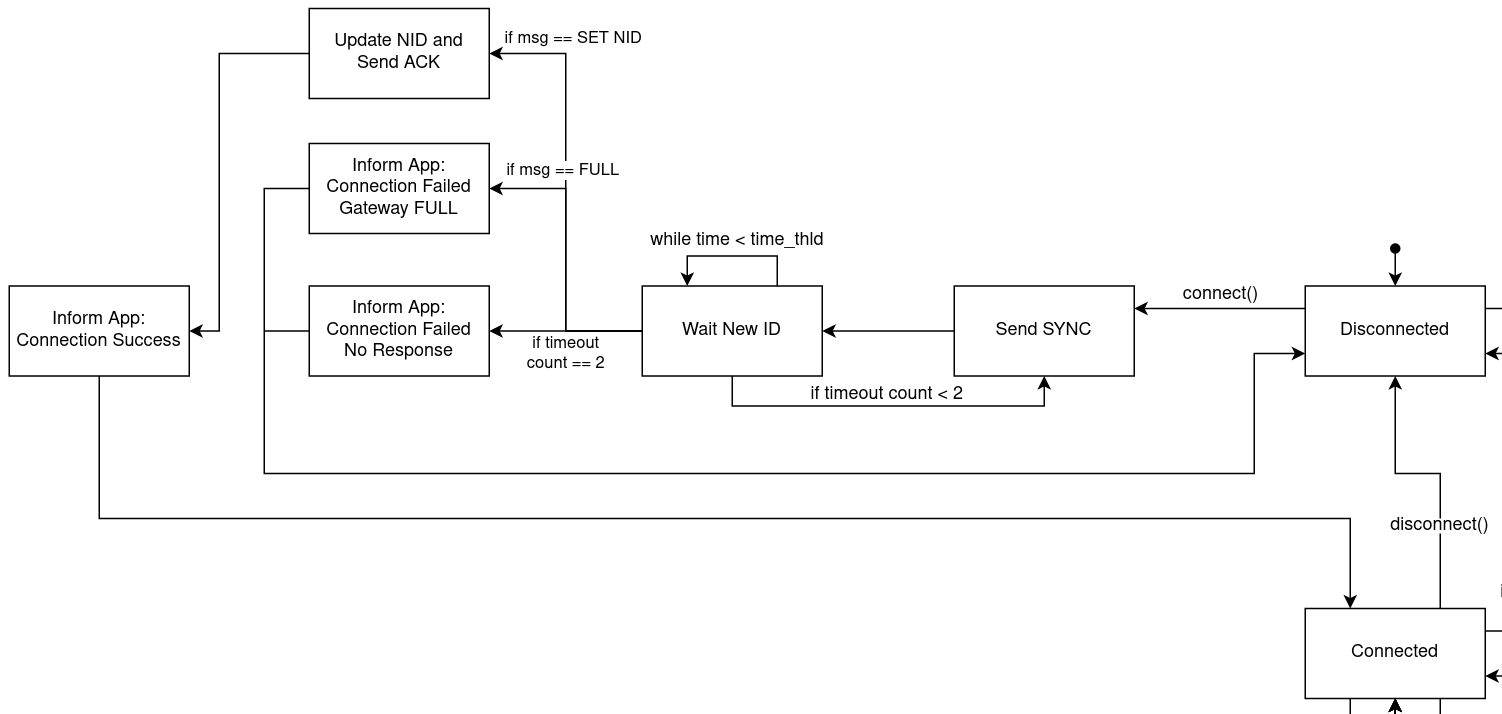
\includegraphics[width=\textwidth,height=0.32\textheight]{img/node-connect.drawio.png}
    Fonte: Autor, 2022.
    \label{fig:fsm-node-connect}
\end{figure}

\begin{figure}[htp]
    \centering
	\caption{Máquina De Estado do Gateway: Conexão com um Gateway}
    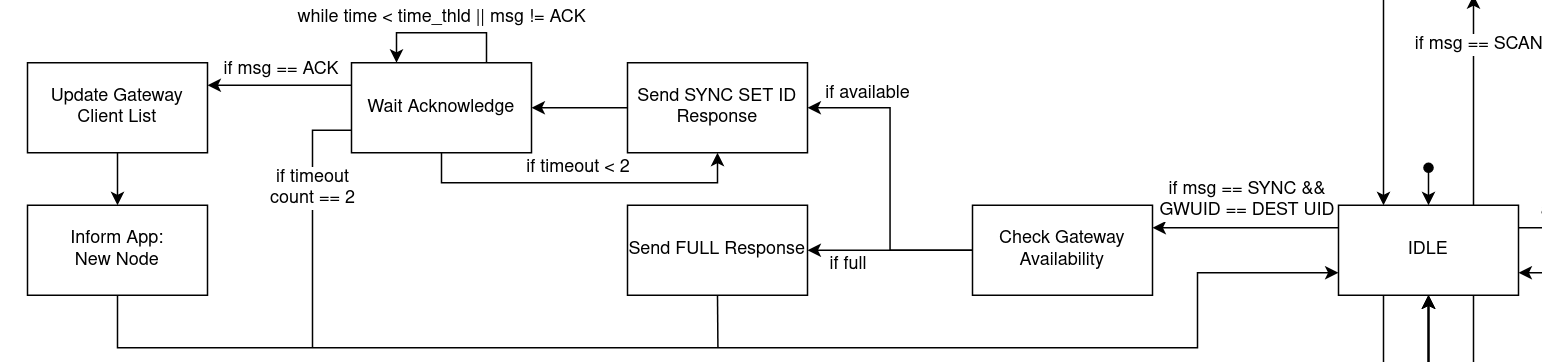
\includegraphics[width=\textwidth]{img/gw-connect.drawio.png}
    
    Fonte: Autor, 2022.
    \label{fig:fsm-gw-connect}
\end{figure}

\newpage

\subsection{Estados de Verificação de Atividade}

Quando um Nó se encontra num estado de conectado, seu UID está
incluso na lista de clientes do Gateways. De tempos em tempos
o Gateway faz uma verificação de atividade de todos seus clientes
para validar que ainda estão comunicáveis dentro da rede. O Gateway
vai para um estado de selecionar o UID do cliente a ser testado,
logo após vai para o estado de envio de sinal de atividade e, por fim,
o estado de espera de confirmação durante determinado tempo.
No Nó, ao estar no estado de conectado
e receber o sinal da verificação de atividade, ele vai para o estado
de resposta ao Gateway que continua comunicável dentro da rede.
Caso o Gateway não receba nenhuma resposta ao seu sinal, ele volta
para o estado de enviar sinal de atividade para tentar mais uma vez.
Caso ainda assim, ele não receba nenhuma resposta, ele vai para o
estado de remoção do NID da lista de clientes, e a partir desse estado
o NID está agora livre para uso em outro cliente que solicitar uma
conexão. Após esse estado, o Gateway volta para o estado de selecionar
um cliente a ser testado, até que não tenha mais nenhum cliente a
testar, logo ele volta pra o estado de espera.

\begin{figure}[htp]
    \centering
	\caption{Máquina De Estado do Nó: Verificação de Atividade}
    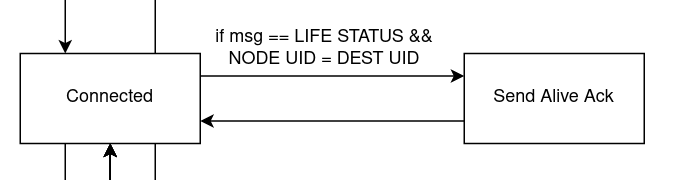
\includegraphics[width=0.6\textwidth]{img/node-alive.drawio.png}
    
    Fonte: Autor, 2022.
    \label{fig:fsm-node-alive}
\end{figure}

\begin{figure}[htp]
    \centering
	\caption{Máquina De Estado do Gateway: Verificação de Atividade}
    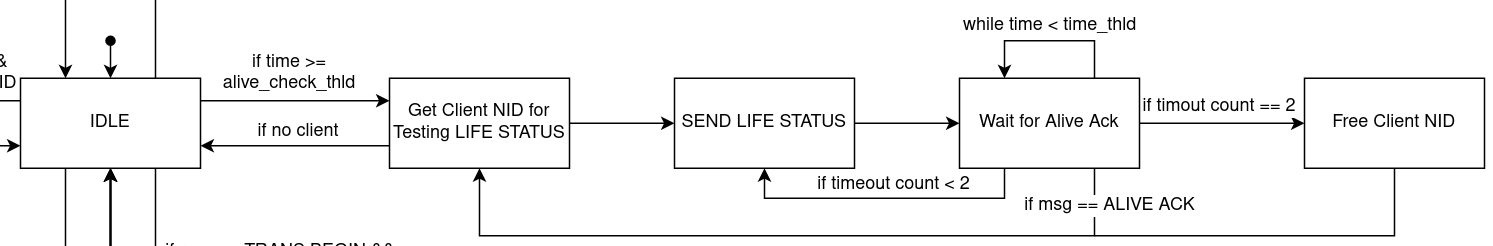
\includegraphics[width=\textwidth]{img/gw-alive.drawio.png}
    
    Fonte: Autor, 2022.
    \label{fig:fsm-gw-alive}
\end{figure}

\subsection{Estados de Envio e Recebimento de Dados}

Os estados de envio e recebimento de dados são comuns para as duas máquinas
implementadas nessa seção. Assim, o fluxo é o mesmo seja um envio do Nó ao
Gateway como do Gateway para o Nó. Ao inciar um fluxo de envio de dados para
um UID especifico, o remetente vai para um estado de dividir os dados em N
pacotes e logo após para o estado de informar o destinatário que deseja fazer
uma transmissão, quantos pacotes pretende enviar, e fica no estado de aguardo.
O destinatário permanece no estado de aguardo até que receba alguma resposta ou
que tenha tentado solicitar a transmissão num total de 2 vezes e mesmo assim não
obteve uma resposta. Já no remetente, ao receber o sinal de solicitação de transmissão,
é feito a mudança para o estado de verificar se existe recursos disponíveis para aceitar
a transmissão, caso sim, é enviado um sinal aceitando a transmissão, caso não, é enviado
um sinal informando que não será possível. A partir desse ponto, tanto o remetente e o
destinatário estão sincronizados para a transmissão, a logica a seguir é, ao envio de cada
pacote, o destinatário precisa acusar o recebimento, caso o recebimento não seja confirmado
o remetente reenvia o mesmo pacote mais uma vez, e se mesmo assim não for confirmado, ele
desistirá da transmissão. Já o destinatário fica no aguardo do pacote com o numero de sequencia
correto, caso ele não receba, ele solicita ao remetente o reenvio desse pacote, se ainda sim ele
não receber, ele desistirá da transmissão. Ao final da transmissão bem sucedida, o destinatário
segue para o estado de reconstrução do dados a partir dos pacotes recebidos e em seguida informa
a aplicação a existência de dados recém chegados.

\begin{figure}[htp]
    \centering
	\caption{Máquina De Estado do Nó: Envio e Recebimento de Dados}
    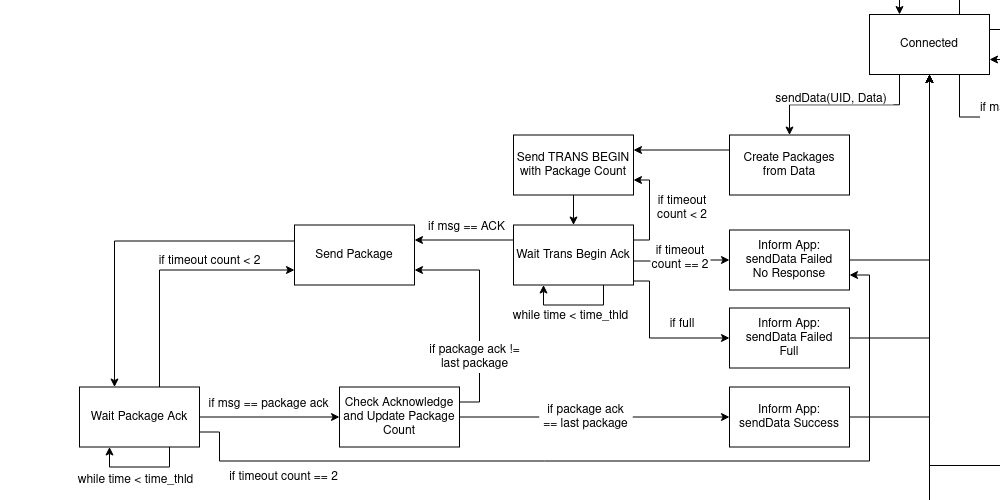
\includegraphics[height=0.27\textheight,keepaspectratio]{img/node-send.drawio.png}
    
    Fonte: Autor, 2022.
    \label{fig:fsm-node-send}
\end{figure}

\begin{figure}[htp]
    \centering
	\caption{Máquina De Estado do Gateway: Envio e Recebimento de Dados}
    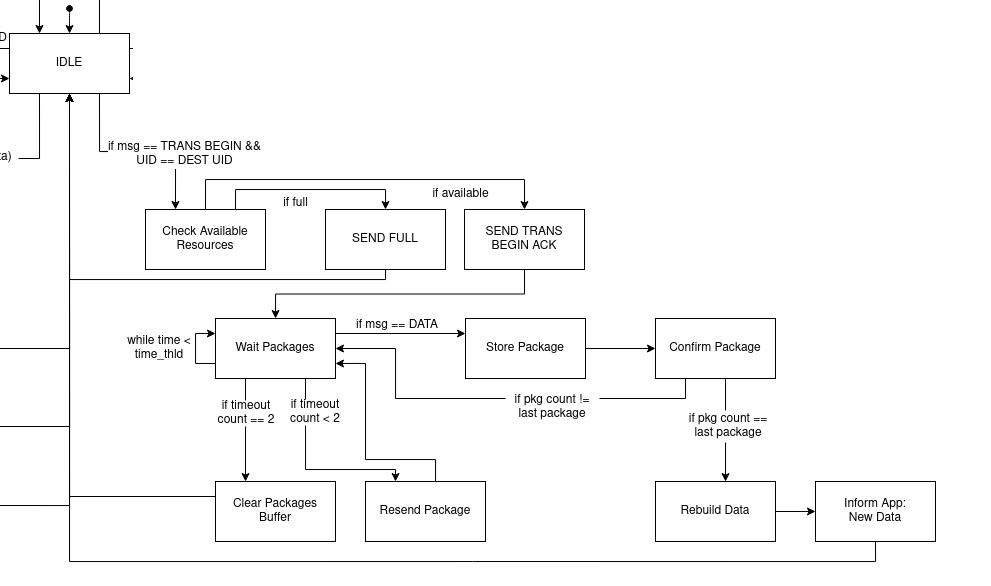
\includegraphics[height=0.28\textheight,keepaspectratio]{img/gw-recv.drawio.png}
    
    Fonte: Autor, 2022.
    \label{fig:fsm-gw-recv}
\end{figure}

\clearpage

\section{Implementação da Arquitetura e Abstração do Hardware}

Esta etapa tem o objetivo de usar de toda documentação gerada na primeira fase
e implementá-la em código executável. Nessa etapa vamos nós preocupar em entender
como o hardware funciona, desde o rádio LoRa aos possíveis microcontroladores, e
as funcionalidades oferecidas por eles e necessárias para a implementação real
da proposta. Para garantir uma boa qualidade de software com códigos bem estruturados
e reutilizáveis, é importante definir um diagrama de blocos da Arquitetura, por meio
do diagrama é possível ver os módulos de software como caixas pretas, a forma que
eles se interagem, os recursos que precisam, e a sua plataforma, que no caso dessa
proposta é o dispositivo embarcado do desenvolvedor IoT. É importante frisar que por
questão de portabilidade, o diagrama representa uma especificação genérica dos softwares
e funcionalidades que podem ser encontradas em vários tipos de dispositivos embarcados,
isso é importante pois garante de certo nível teórico que o protocolo pode ser implementado
apenas uma vez e portado para vários dispositivos.

\subsection{Diagrama de Blocos}

\begin{figure}[h]
    \centering
	\caption{Diagrama macro do Hardware e Software}
    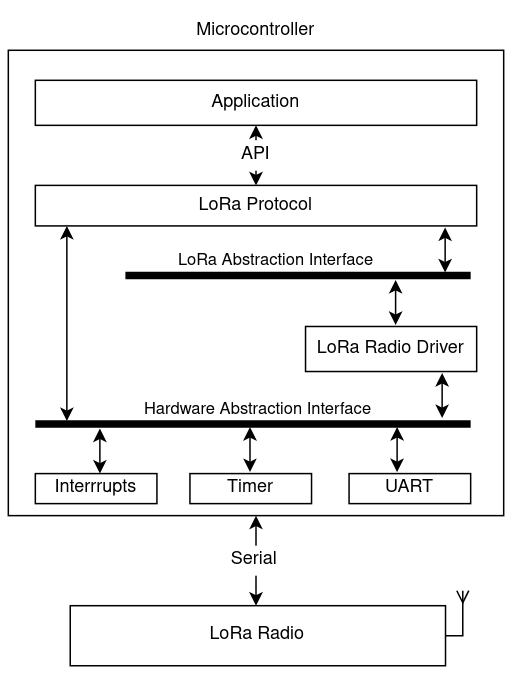
\includegraphics[width=0.5\textwidth,height=0.5\textheight,keepaspectratio]{img/blk.drawio.png}
    \label{fig:blk}
    
    Fonte: Autor, 2022.
\end{figure}

O Diagrama de Blocos definido na Figura \ref{fig:blk} representa a estrutura de software
definida para esse trabalho. A aplicação conversa com o protocolo por meio de uma API
(Application Progamming Interface) que por sua vez utiliza recursos do hardware por
meio de camadas de abstração, chamadas de \textit{Interfaces}, que por sua vez chamam 
as funções específicas do hardware a ser utilizado.
Dessa forma, mesmo que o hardware e/ou rádio LoRa mudem, não é necessário refatorar
nenhuma parte do código do protocolo. Nas próximas sub-seção será melhor descrito como
foi atingida essa abstração nesse trabalho.

\subsection{Módulos internos do Protocolo}

O protocolo possui 5 componentes extremamente importantes para garantir uma boa modularização,
uma boa utilização dos recursos de hardware, e mais importante ainda, garantir todas as funcionalidades
descritas nas documentações, nessa sub-seção vamos entrar em detalhes sobre esses componentes. Na
figura \ref{fig:gw-blk} a seguir é possível visualizar esses 5 módulos que compõe o módulo final do
Gateway.

\begin{figure}[H]
    \centering
	\caption{Diagrama micro do modulo do protocolo para o Gateway}
    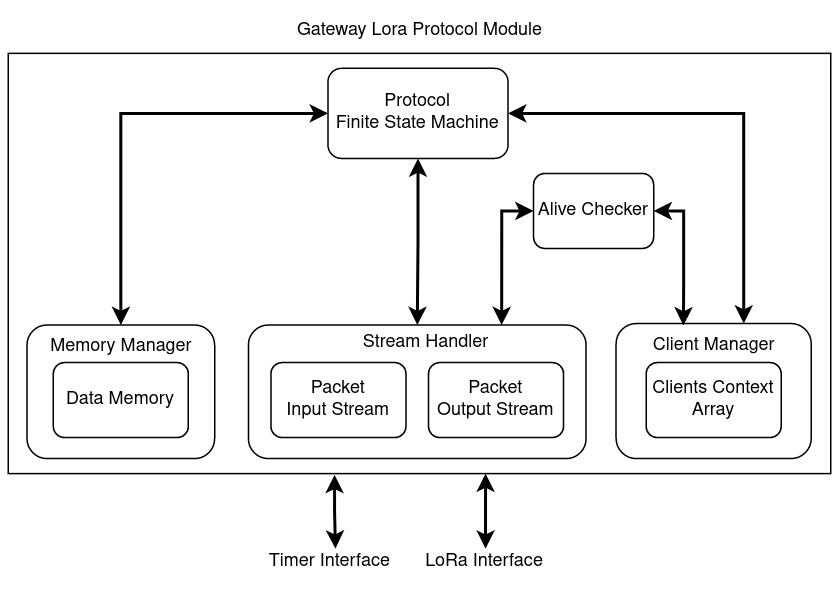
\includegraphics[height=0.3\textheight,keepaspectratio]{img/gw-block.drawio.png}
    \label{fig:gw-blk}
    
    Fonte: Autor, 2022.
\end{figure}

\subsubsection{Stream Handler}

O stream handler é um modulo para gerenciar os pacotes que estão indo e vindo pelo protocolo,
ele possui duas filas circulares, uma para os pacotes de entrada, e uma para os pacotes de saída,
sua função principal é de ordenar a ordem de tratamento dos pacotes e servir como um buffer temporário
enquanto a maquina de estado estiver ocupada. Na figura \ref{fig:code-sh} é possível ver a implementação
do modulo.

\begin{figure}[H]
    \centering
	\caption{Código do Stream Handler}
    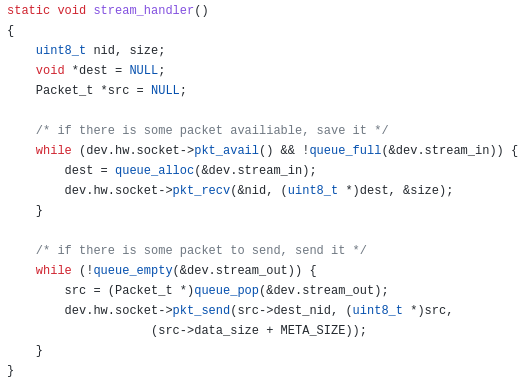
\includegraphics[height=0.3\textheight,keepaspectratio]{img/stream-handler.png}
    \label{fig:code-sh}
    
    Fonte: Autor, 2022.
\end{figure}

\subsubsection{Client Manager}

O client manager é um conjunto de APIs usadas pela maquina de estado e pelo modulo de Alive Checker
para interagir com uma área de memoria responsável por guardar informações criticas para cada conexão,
essa área de memoria é um array com indexação baseada no NID do cliente. Na figura \ref{fig:code-clt-ctx} a seguir é possível ver os dados armazenados para cada entrada desse array.

\begin{figure}[H]
    \centering
	\caption{Dados de uma entrada do array de clientes}
    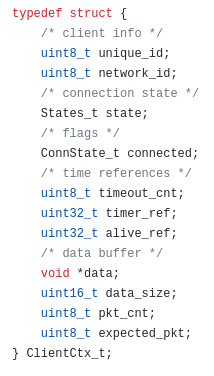
\includegraphics[height=0.3\textheight,keepaspectratio]{img/clt-ctx.png}
    \label{fig:code-clt-ctx}
    
    Fonte: Autor, 2022.
\end{figure}

\subsubsection{Alive Checker}

O alive checker é o modulo responsável por estar sempre analisando a lista de clientes e
validando a se algum cliente passou muito tempo sem se comunicar, dependendo do tempo limite
configurado, ele testará cada cliente que passar desse limiar. Na figura \ref{fig:code-alive-checker} a seguir é possível ver sua implementação.

\begin{figure}[H]
    \centering
	\caption{Código do Alive Checker}
    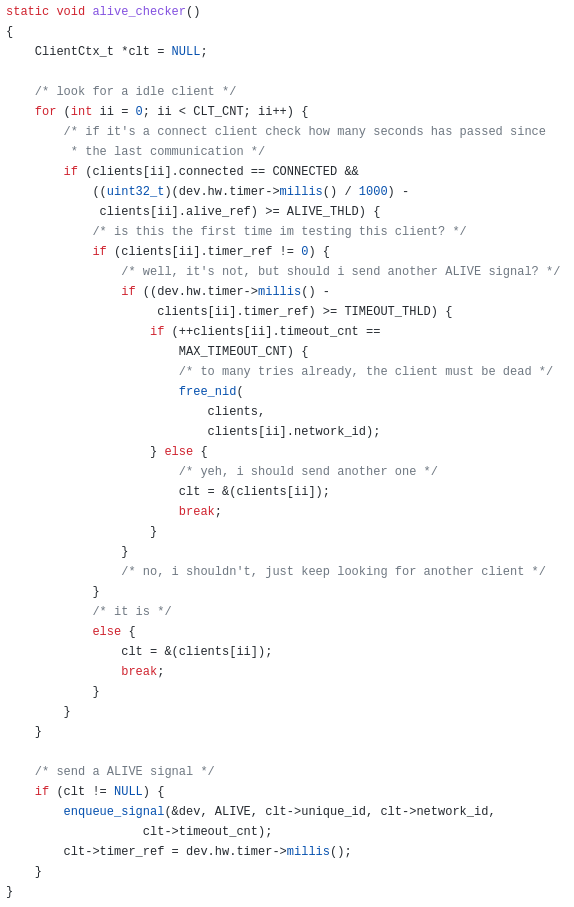
\includegraphics[height=0.7\textheight,keepaspectratio]{img/alive-checker.png}
    \label{fig:code-alive-checker}
    
    Fonte: Autor, 2022.
\end{figure}

\subsubsection{Memory Manager}

o memory manager é o modulo que implementa algoritmos de alocação dinâmica de um determinado espaço
continuo de memoria. O memory manager é um modulo extramente pois é a partir dele que o Gateway consegue
ter diferentes espaços de memoria reservados para as diferentes transmissões de dados simultâneas que possam acontecer. Com isso é possível garantir que o protocolo use uma quantidade especifica de memoria do hardware mas que será gerenciada de maneira inteligente para diferentes recursos. Na figura \ref{fig:code-memmgr-api} a seguir é possível ver as APIs do memory manager.

\begin{figure}[H]
    \centering
	\caption{APIs do Memory Manager}
    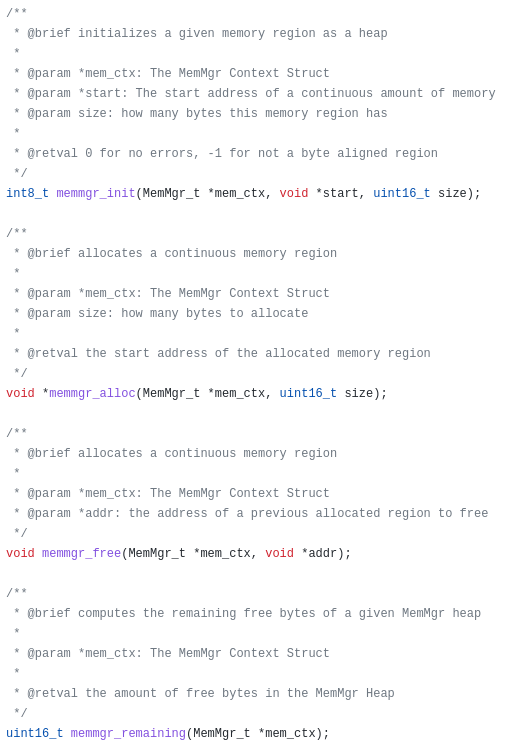
\includegraphics[height=0.55\textheight,keepaspectratio]{img/memmgr-api.png}
    \label{fig:code-memmgr-api}
    
    Fonte: Autor, 2022.
\end{figure}

\subsubsection{Protocol Finite State Machine}

A maquina de estado implementada é o maior modulo em relação a linhas de código, ela que
garantes as funcionalidades e fluxos definidos nas etapas de documentação. Sua implementação
é a tradução direta para código do que foi documento na etapa de geração das maquinas de estado.

\subsubsection{Juntando os componentes}

Com isso, o modulo macro do procolo foi definido numa estrutura que pode ser vista na figura \ref{fig:dev}
e sua inicialização na figura \ref{fig:gw-init}.

\begin{figure}[H]
    \centering
	\caption{Estrutura do protocolo macro}
    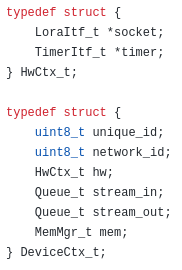
\includegraphics[height=0.2\textheight,keepaspectratio]{img/dev.png}
    \label{fig:dev}
    
    Fonte: Autor, 2022.
\end{figure}

\begin{figure}[H]
    \centering
	\caption{Inicialização da estrutura do protocolo macro}
    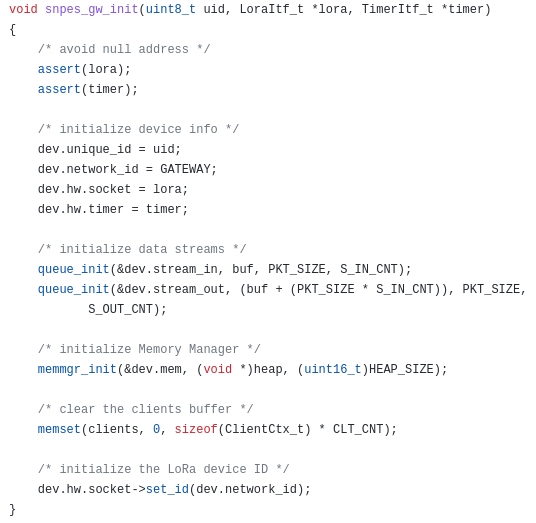
\includegraphics[height=0.4\textheight,keepaspectratio]{img/gw-init.png}
    \label{fig:gw-init}
    
    Fonte: Autor, 2022.
\end{figure}

\subsection{Removendo as dependências do Hardware}

No geral, recursos de hardware, seja qual for a arquitetura, são acessados
por meio de leituras e escritas em endereços de memória específicos. Esses
endereços recebem uma nomenclatura especial de \textit{Registradores}. De maneira
simples, um programador que deseja mudar o estado de um pino numa porta
GPIO entre HIGH e LOW, basta mudar o bit que representa o pino
de interesse no registrador da porta GPIO. Apesar da teoria ser a mesma
para muitos casos de microcontroladores, a pratica não é, pois os registradores
diferem de estrutura e endereço de arquitetura para arquitetura.

Isso implica que, ao desenvolver alguma funcionalidade que utilize recursos
do hardware, ela teria que ser rescrita para cada arquitetura final, algo
totalmente impraticável se o objetivo é suportar diferentes hardwares. Como
solução para esse problema surgiu o conceitos de \textit{Interfaces}

\subsubsection{Abstração com Interfaces}

Interfaces é um conceito extramente usado no kernel Linux, em outros sistemas
operacionais e firmwares para obter abstração e modularização. Uma interface
é simplesmente uma \textbf{estrutura} que \textbf{descreve} funcionalidades. Por exemplo,
uma transmissão serial possui as \textbf{funcionalidades} de \textit{escrever}
e \textit{ler} bytes por um determinado canal, funções mais alto nível que desejam
utilizar essas funcionalidades podem ter como \textbf{dependência} a interface
que as definem. Dessa forma, é possível que para cada mudança de hardware
seja apenas necessário atualizar quais funções especificas essa interface apontará,
e com isso nenhuma mudança de código será necessária já que as funções mais alto
nível \textbf{dependem} da interface e sua definição nunca muda. Nas figuras
\ref{fig:itf-timer} e \ref{fig:itf-lora} a seguir é possui visualizar em código as interfaces
definidas nesse projeto para as funcionalidades de Timer e Rádio loRa respectivamente.

\begin{figure}[H]
    \centering
	\caption{Interface Timer}
    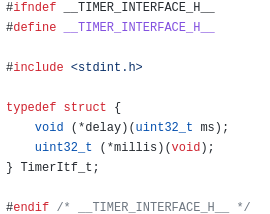
\includegraphics[height=0.19\textheight,keepaspectratio]{img/itf-timer.png}
    \label{fig:itf-timer}
    
    Fonte: Autor, 2022.
\end{figure}

\begin{figure}[H]
    \centering
	\caption{Interface LoRa}
    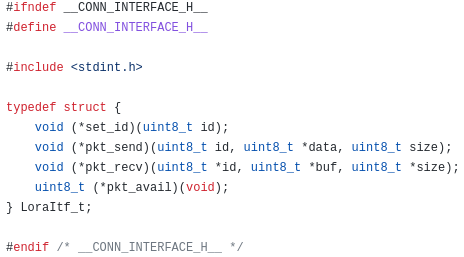
\includegraphics[height=0.2\textheight,keepaspectratio]{img/itf-lora.png}
    \label{fig:itf-lora}
    
    Fonte: Autor, 2022.
\end{figure}

\newpage

Pelas figuras é possível ver que as interfaces são simplesmente um conjunto
de ponteiros que direcionam para as funções dependentes do hardware. Na figura
\ref{fig:gw-init-def} a seguir é possível visualizar que o protocolo depende dessas interfaces.
E nas figuras \ref{fig:timer-ex} e \ref{fig:lora-ex} é possível visualizar
exemplos de uso dessas interfaces.

\begin{figure}[H]
    \centering
	\caption{Assinatura de função de inicialização do Protocolo}
    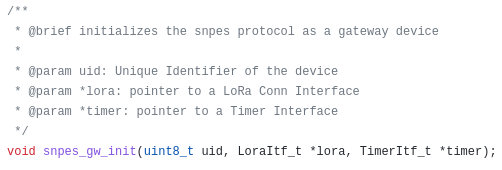
\includegraphics[height=0.14\textheight,keepaspectratio]{img/gw-init-def.png}
    \label{fig:gw-init-def}
    
    Fonte: Autor, 2022.
\end{figure}

\begin{figure}[H]
    \centering
	\caption{Exemplo de uso da Interface Timer}
    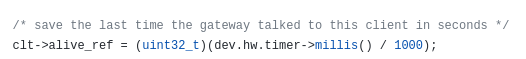
\includegraphics[width=0.7\textwidth,keepaspectratio]{img/timer-ex.png}
    \label{fig:timer-ex}
    
    Fonte: Autor, 2022.
\end{figure}

\begin{figure}[H]
    \centering
	\caption{Exemplo de uso da Interface LoRa}
    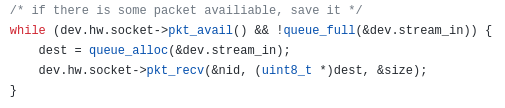
\includegraphics[height=0.09\textheight,keepaspectratio]{img/lora-ex.png}
    \label{fig:lora-ex}
    
    Fonte: Autor, 2022.
\end{figure}

\newpage

\subsection{Implementação final}

A implementação final do projeto ficou de acordo com a tabela \ref{tab:files} a seguir
e pode ser publicamente acessada na url: \url{https://github.com/mfbsouza/snpes}. O projeto
final ganhou o apelido de "SNPES" [isnepis] que significa Simple Network Protocol for Embedded
Systems.  

\begin{longtable}{|l|l|l|}
    \caption{Arquivos de código do Projeto}\label{tab:files}\\
    \hline
    \textbf{Pasta} & \
    \textbf{Arquivo} & \
    \textbf{Qnt. de linhas} \\
    \cline{1-3}
    src & \
    CircularQueue.c & \
    123 \\
    \cline{2-3}
     & \
    CircularQueue.h & \
    90 \\
    \cline{2-3}
     & \
    ConnInterface.h & \
    13 \\
    \cline{2-3}
     & \
    MemoryManager.c & \
    113 \\
    \cline{2-3}
     & \
    MemoryManager.h & \
    60 \\
    \cline{2-3}
     & \
    snpes\_cfg.h & \
    49 \\
    \cline{2-3}
     & \
    snpes\_gateway.c & \
    351 \\
    \cline{2-3}
     & \
    snpes\_gateway.h & \
    49 \\
    \cline{2-3}
     & \
    snpes\_node.c & \
    186 \\
    \cline{2-3}
     & \
    snpes\_node.h & \
    55 \\
    \cline{2-3}
     & \
    snpes\_types.h & \
    88 \\
    \cline{2-3}
     & \
    snpes\_utils.c & \
    128 \\
    \cline{2-3}
     & \
    snpes\_utils.h & \
    122 \\
    \cline{2-3}
     & \
    TimerInterface.h & \
    11 \\
    \hline
    
    tests & \
    AllTests.cpp & \
    6 \\
    \cline{2-3}
     & \
    CircularQueueTests.cpp & \
    166 \\
    \cline{2-3}
     & \
    MemoryManagerTests.cpp & \
    117 \\
    \cline{2-3}
     & \
    SnpesGatewayTests.cpp & \
    532 \\
    \cline{2-3}
     & \
    SnpesNodeTests.cpp & \
    248 \\
    \cline{2-3}
     & \
    SnpesUtilsTests.cpp & \
    150 \\
    \hline
    
    Total & \
     & \
    2657 \\
    \hline
\end{longtable}